% !TEX program = xelatex
\documentclass[12pt,a4paper]{report}

%% ─── Packages ─────────────────────────────────────────────────────────────────
\usepackage{fontspec}
\setmainfont{Times New Roman}
\usepackage{xcolor}            % must come BEFORE hyperref — enables blue!60!black mixing
\usepackage{polyglossia}
\setmainlanguage{english}
\setotherlanguage{arabic}
\newfontfamily\arabicfont[Script=Arabic, Scale=1.1]{Times New Roman}
\newcommand{\lr}[1]{\textenglish{#1}}
\usepackage{geometry}
\usepackage{graphicx}
\usepackage{array}
\usepackage{booktabs}
\usepackage{longtable}
\usepackage{tabularx}
\usepackage{enumitem}
\usepackage{hyperref}
\usepackage{setspace}
\usepackage{xurl}
\usepackage{microtype}
\usepackage{pdfpages}
\usepackage{pdflscape}
\usepackage{csquotes}          % required by biblatex (proper multilingual quoting)
\usepackage[
  backend    = biber,          % use biber (not bibtex) for full Unicode + DOI support
  style      = numeric,        % [1], [2], … citation labels
  citestyle  = numeric-comp,   % compressed: [1–3] instead of [1,2,3]
  sorting    = none,           % references appear in citation order
  maxbibnames= 6,              % truncate author lists longer than 6
  minbibnames= 3,              % keep at least 3 before "et al."
  url        = true,
  doi        = true,
  isbn       = false,
  date       = year,           % show only the year in the bibliography
]{biblatex}
\addbibresource{pfebiblio.bib}

%% ─── Page geometry ─────────────────────────────────────────────────────────────
\geometry{top=2.5cm, bottom=2.5cm, left=2.5cm, right=2.5cm}
\onehalfspacing
\setlist[itemize]{label=--, leftmargin=1.2cm}

%% ─── Hyperref setup ────────────────────────────────────────────────────────────
\hypersetup{
  colorlinks  = true,
  linkcolor   = blue!60!black,
  urlcolor    = blue!70!black,
  citecolor   = blue!60!black,
  pdftitle    = {EV Charge Manager -- MFE Fodhil \& Chibani},
  pdfauthor   = {Yacine FODHIL, Abderrahmane CHIBANI},
}

\renewcommand{\contentsname}{Table of Contents}

%%%=============================================================================
\begin{document}

%% ─── TITLE PAGE ───────────────────────────────────────────────────────────────
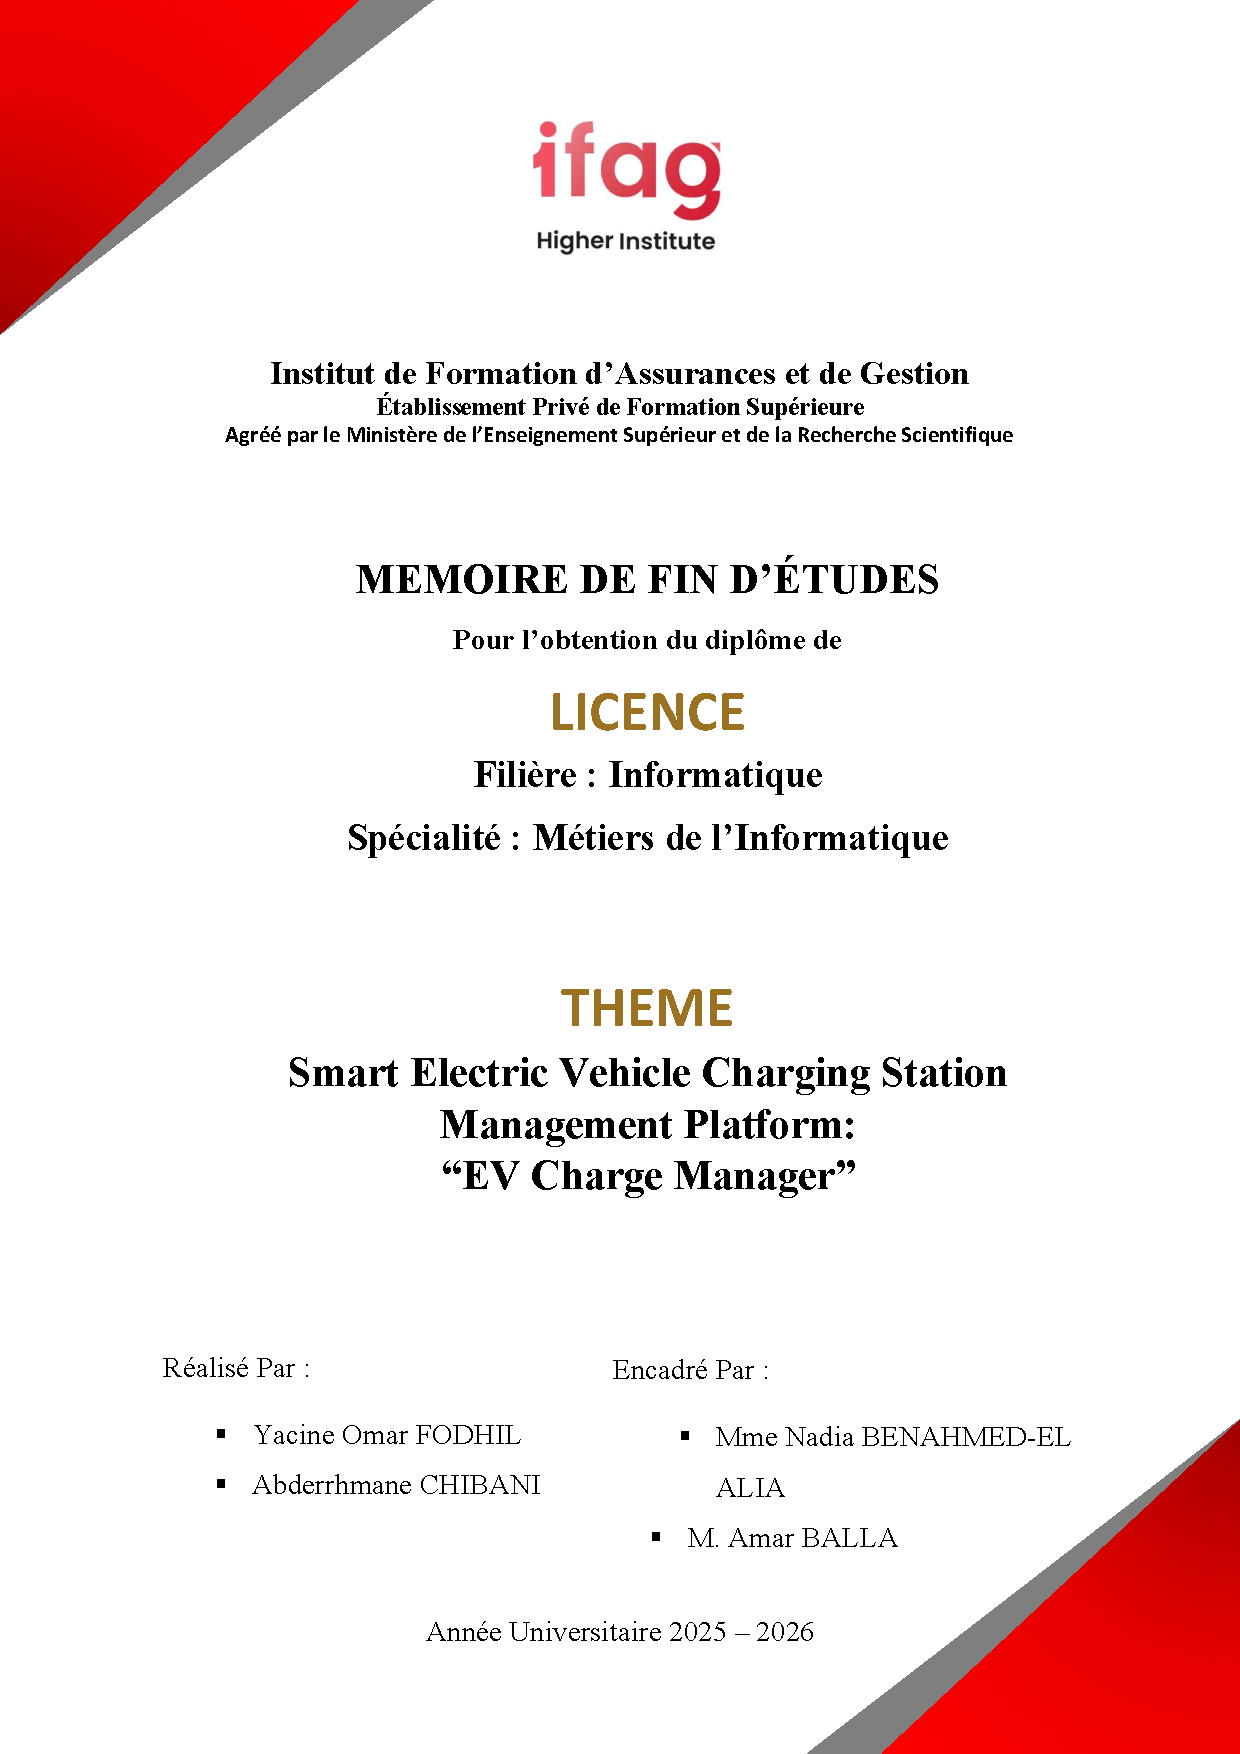
\includepdf[pages=1,fitpaper=true]{page_garde.pdf}

%%%=============================================================================
%%  FRONT MATTER
%%%=============================================================================
\hypersetup{pageanchor=false}
\pagenumbering{roman}

\chapter*{Dedication}
\addcontentsline{toc}{chapter}{Dedication}

To our parents, who sacrificed so much and, at times, everything, so that we could reach this
level. Your unwavering love, endless patience, and constant support were the foundation upon
which we built our journey. You were our light in moments of doubt and our strength when the
path felt difficult.

To our brothers and sisters, whose daily presence, encouragement, and belief in us made every
challenge feel lighter. Your words, smiles, and support were a quiet but powerful source of
motivation.

To ourselves, for our sincere collaboration, our discipline, and our commitment throughout this
project. Through moments of pressure, late nights, and shared efforts, we proved that
perseverance and teamwork lead to achievement.

To all our friends and classmates, with whom we shared not only knowledge but also unforgettable
moments, laughter, and challenges. This academic journey would not have been the same without
you, and these memories will remain with us far beyond this project.

% ──────────────────────────────────────────────────────────────────────────────
\chapter*{Acknowledgments}
\addcontentsline{toc}{chapter}{Acknowledgments}

First and foremost, we thank Allah, the Almighty, for granting us the strength, patience, and
perseverance to complete this work. Without His will, none of this would have been possible.

We would also like to express our deepest gratitude to our parents and family for their
sacrifices, unconditional support, constant encouragement, and unwavering belief in us
throughout our journey. Their presence has been a true source of motivation and comfort.

We extend our heartfelt appreciation to our teachers, whose guidance has been invaluable:

To Mr.\ Balla, who was more than a teacher to us---he was like a father. His wisdom, constant
support, and sincere care guided us not only academically but also personally. He believed in
us, encouraged us in difficult moments, and inspired us to always strive for better.

To Mrs.\ BENAHMED-EL ALIA, who embodied the role of a caring and guiding mother. Her kindness,
patience, and dedication created a supportive environment where we felt encouraged to grow,
learn, and express ourselves with confidence.

To Mr.\ Mokeddem, who provided us with a strong foundation in understanding development. His
clarity, guidance, and generosity in sharing knowledge helped us build solid academic skills
and a deeper way of thinking.

We would also like to express our sincere thanks to Mr.\ Chagroune for his warm welcome at
SAIEG, his honest guidance, and the valuable information he generously shared with us.

We are truly grateful for their dedication, support, and the lasting impact they have had on
our journey.

% ──────────────────────────────────────────────────────────────────────────────
\chapter*{Résumé / Abstract}
\addcontentsline{toc}{chapter}{Résumé / Abstract}

\section*{Résumé (Français)}

EV Charge Manager est une plateforme web multi-tenant dédiée à la gestion de l'infrastructure
de recharge pour véhicules électriques (VE) en Algérie. Face à l'expansion progressive de la
mobilité électrique et à l'absence de solutions logicielles adaptées au contexte réglementaire
et infrastructurel algérien, ce projet vise à fournir un système de gestion complet, robuste
et évolutif.

La plateforme offre une interface opérationnelle unifiée couvrant la gestion du cycle de vie
des bornes de recharge, la supervision des sessions de charge, le traitement de la facturation,
la gestion des tickets de maintenance et l'administration des droits d'accès. Elle repose sur
le protocole Open Charge Point Protocol~1.6 (OCPP~1.6) pour la communication avec les
équipements physiques et adopte une architecture trois tiers : une application web
React~18/TypeScript, une API REST Node.js/Express.js, et une base de données MySQL~8.

Le modèle multi-tenant garantit une isolation complète des données entre opérateurs
indépendants, avec un contrôle d'accès granulaire fondé sur les rôles (RBAC). Un mécanisme
de dégradation gracieuse assure la continuité d'exploitation en mode hors ligne.

Les résultats obtenus démontrent la faisabilité d'une solution de gestion de bornes adaptée
au marché algérien, constituant une base technique solide pour un déploiement à grande échelle.

\medskip
\noindent\textbf{Mots-clés~:} véhicule électrique, gestion de bornes de recharge, OCPP~1.6,
architecture multi-tenant, RBAC, React, Node.js, Algérie.

\bigskip
\section*{Abstract (English)}

EV Charge Manager is a multi-tenant web platform designed to manage electric vehicle~(EV)
charging infrastructure in Algeria. In response to the progressive electrification of the
Algerian automotive sector and the absence of purpose-built management software adapted to
the local regulatory environment, this project delivers an integrated, scalable, and robust
charging management system.

The platform provides a unified operational interface covering station lifecycle management,
session monitoring, billing processing, maintenance ticket management, and user access
administration. It communicates with physical hardware using the Open Charge Point
Protocol~1.6~(OCPP~1.6) and follows a three-tier architecture comprising a React~18/TypeScript
single-page application, a Node.js/Express.js REST API, and a MySQL~8 relational database.

The multi-tenant model enforces complete data isolation between independent operators through
role-based access control~(RBAC) with fine-grained privilege management. A graceful degradation
strategy ensures operational continuity during network failures through browser-side caching.

The results demonstrate the feasibility of a locally adapted EV charging management solution,
establishing a solid technical foundation for large-scale deployment in the Algerian market.

\medskip
\noindent\textbf{Keywords:} electric vehicle, EV charging management, OCPP~1.6, multi-tenant
architecture, RBAC, React, Node.js, Algeria.

\bigskip
\begin{Arabic}
\section*{ملخص (بالعربية)}

\lr{EV Charge Manager} هي منصة ويب متعددة المستأجرين (\lr{Multi-Tenant}) مخصصة لإدارة
البنية التحتية لشحن المركبات الكهربائية في الجزائر. في ظل التوسع التدريجي للتنقل الكهربائي
وغياب الحلول البرمجية الملائمة للسياق التنظيمي والبنيوي الجزائري، يهدف هذا المشروع إلى
توفير نظام إدارة شامل وموثوق وقابل للتطوير.

تُقدّم المنصة واجهة تشغيلية موحّدة تشمل إدارة دورة حياة محطات الشحن، والإشراف على جلسات
الشحن، ومعالجة الفواتير، وإدارة تذاكر الصيانة، وضبط صلاحيات الوصول. وتعتمد على بروتوكول
\lr{Open Charge Point Protocol 1.6 (OCPP 1.6)} للتواصل مع الأجهزة الفيزيائية، وتتبنى
معمارية ثلاثية الطبقات تتكون من: تطبيق ويب مبني بـ\lr{React 18/TypeScript}، وواجهة برمجية
\lr{REST API} مبنية بـ\lr{Node.js/Express.js}، وقاعدة بيانات \lr{MySQL 8}.

يضمن النموذج متعدد المستأجرين عزلاً كاملاً للبيانات بين المشغّلين المستقلين، مع تحكم دقيق
في الوصول مبني على الأدوار (\lr{RBAC}). كما يتضمن النظام آلية تدهور رشيق تكفل استمرارية
التشغيل في وضع عدم الاتصال.

تُثبت النتائج المحققة جدوى حل إدارة محطات الشحن المتكيّف مع السوق الجزائرية، مما يُشكّل
أساساً تقنياً متيناً لنشره على نطاق واسع.

\medskip
\noindent\textbf{الكلمات المفتاحية:} المركبة الكهربائية، إدارة محطات الشحن،
\lr{OCPP 1.6}، معمارية متعددة المستأجرين، \lr{RBAC}، \lr{React}، \lr{Node.js}، الجزائر.
\end{Arabic}

% ──────────────────────────────────────────────────────────────────────────────
\tableofcontents
\listoffigures
\listoftables

% ──────────────────────────────────────────────────────────────────────────────
\chapter*{List of Abbreviations}
\addcontentsline{toc}{chapter}{List of Abbreviations}

\begin{longtable}{>{\bfseries}p{3.2cm} p{10.5cm}}
  API    & Application Programming Interface \\
  CC     & Constant Current \\
  CIB    & Carte Interbancaire (Algerian bank card) \\
  CPO    & Charge Point Operator \\
  CSMS   & Charging Station Management System \\
  CV     & Constant Voltage \\
  DZD    & Algerian Dinar \\
  EIM    & External Identification Means \\
  EV     & Electric Vehicle \\
  EVCC   & Electric Vehicle Communication Controller \\
  EVSE   & Electric Vehicle Supply Equipment \\
  HMI    & Human-Machine Interface \\
  HTTP   & Hypertext Transfer Protocol \\
  IEC    & International Electrotechnical Commission \\
  IoT    & Internet of Things \\
  ISO    & International Organization for Standardization \\
  JSON   & JavaScript Object Notation \\
  JWT    & JSON Web Token \\
  KPI    & Key Performance Indicator \\
  OCPP   & Open Charge Point Protocol \\
  OTP    & One-Time Password \\
  PnC    & Plug \& Charge \\
  PV     & Photovoltaic \\
  RBAC   & Role-Based Access Control \\
  REST   & Representational State Transfer \\
  RFID   & Radio-Frequency Identification \\
  RISE V2G & Robust Implementation and Standardized Extensions for V2G \\
  SaaS   & Software as a Service \\
  SECC   & Supply Equipment Communication Controller \\
  SLA    & Service Level Agreement \\
  SoC    & State of Charge \\
  SPA    & Single-Page Application \\
  TLS    & Transport Layer Security \\
  V2G    & Vehicle-to-Grid \\
\end{longtable}

\clearpage
\hypersetup{pageanchor=true}
\pagenumbering{arabic}

%%%=============================================================================
%%  GENERAL INTRODUCTION
%%%=============================================================================

\chapter*{General Introduction}
\addcontentsline{toc}{chapter}{General Introduction}

The rapid global expansion of electric vehicle (EV) adoption has created an urgent need for
robust, intelligent charging infrastructure management systems. According to the International
Energy Agency, the global EV fleet surpassed 40 million vehicles in 2023, with continued
exponential growth projected through the decade~\autocite{iea_ev_outlook_2024}. This transformation
demands not only physical charging hardware but also sophisticated software platforms capable of
managing stations, monitoring sessions, processing payments, and coordinating maintenance
operations at scale.

In Algeria, where the automotive sector is undergoing gradual electrification, operators such as
Sonelgaz (the national electricity provider) and private partners are beginning to deploy EV
charging networks. However, the absence of purpose-built management software tailored to the
Algerian regulatory environment and infrastructure context represents a significant barrier to
scaled deployment. This gap in the local market constitutes the central problematic that this
work seeks to address.

This thesis presents \textbf{EV Charge Manager}, a multi-tenant web platform developed to address
these challenges. The platform provides a comprehensive operational interface for managing charging
stations, monitoring sessions, handling maintenance tickets, and processing billing records. It
communicates with physical hardware using the Open Charge Point Protocol~1.6
(OCPP~1.6)~\autocite{ocpp16_ed2} and is built on modern open-source web technologies, with a
deployment target adapted to the Algerian market.

The work is organized as follows:

\begin{itemize}
  \item \textbf{Chapter~1} constitutes the first part of the state of the art. It examines the
        ISO~15118 standard, which defines the vehicle-to-grid communication interface and underpins
        advanced charging features such as Plug\,\&\,Charge and demand
        response~\autocite{iso15118_2022}.

  \item \textbf{Chapter~2} completes the state of the art with a comparative analysis of
        OCPP~1.6 and OCPP~2.0, justifies the protocol choice for this project in the Algerian
        context, and surveys existing EV charging management
        platforms~\autocite{ocpp16_ed2, ocpp201}.

  \item \textbf{Chapter~3} presents the requirements analysis for EV Charge Manager, identifying
        the system actors, specifying functional and non-functional requirements, and establishing
        the use cases and technical constraints that frame the design.

  \item \textbf{Chapter~4} details the architectural and design decisions of the platform,
        covering the three-tier architecture, multi-tenant isolation model, data model, access
        control structure, and authentication flow.

  \item \textbf{Chapter~5} presents the concrete implementation of all functional modules and
        demonstrates the operational behaviour of the deployed platform.
\end{itemize}

\medskip
\noindent\textbf{Declaration on the use of AI tools.} During the realization of this work,
AI-assisted tools --- specifically Claude~AI (Anthropic) --- were used to support documentation
drafting and code debugging. All content has been reviewed, corrected, and contextualised by
the authors, who take full responsibility for the accuracy, originality, and integrity of this
report.

\clearpage

%%%=============================================================================
%%  PARTIE I — ÉTAT DE L'ART
%%%=============================================================================

\part*{État de l'Art}
\addcontentsline{toc}{part}{État de l'Art}

%%%=============================================================================
%%  CHAPTER 1 — ISO 15118
%%%=============================================================================

\chapter{ISO~15118 Standard --- Definition \& Application in the EV Charging Platform}

This chapter presents the ISO~15118 international standard, which governs the communication
interface between electric vehicles and charging infrastructure. We examine its definition,
its relevance to smart EV charging, and its concrete application within the context of this
project, covering the system architecture, charging modes, dynamic parameter exchange, demand
response, IoT integration, and security mechanisms.

\section{What is ISO~15118?}

ISO~15118 is an international standard that defines the communication interface between an
Electric Vehicle (EV) and Electric Vehicle Supply Equipment (EVSE)---commonly known as a
charging station~\autocite{iso15118_2022}. It is officially titled \textit{``Road Vehicles---Vehicle
to Grid Communication Interface''} and is developed by the International Organization for
Standardization (ISO).

The standard goes far beyond simple plug-and-charge detection. It establishes a full bidirectional
digital communication protocol---referred to as Vehicle-to-Grid (V2G) communication---enabling EVs
and charging infrastructure to exchange rich data in real time. This includes authentication,
charge parameter negotiation, energy management, and support for grid services. The potential of
V2G for grid stabilisation has been extensively studied: Yilmaz and Krein~\autocite{yilmaz2013}
demonstrated significant benefits in grid stability and utility revenue from managed EV charging.

ISO~15118 is structured across multiple parts (Parts~1--20), covering physical layer requirements,
network and transport layers, application layer messaging, and security. The version most relevant
to practical implementations is \textbf{ISO~15118-2}, which defines the application-layer message
set used during a charging session~\autocite{iso15118_2022}.

% ──────────────────────────────────────────────────────────────────────────────
\section{Why ISO~15118 Matters for Smart EV Charging}

Before ISO~15118, EV charging relied on the IEC~61851-1 standard~\autocite{iec61851_2017}, which uses
simple low-level control pilot signaling. This approach only communicates two pieces of information:
whether a vehicle is connected, and what maximum current the charger can supply. This severely
limits smart charging capabilities.

ISO~15118 addresses these limitations by enabling:

\begin{itemize}
  \item \textbf{Plug \& Charge (PnC):} The EV is automatically identified and authorized using
        digital certificates, eliminating the need for RFID cards or apps.

  \item \textbf{Bidirectional Communication:} Both the EV and EVSE can send and receive detailed
        parameters such as State of Charge (SoC), target current/voltage, and power limits.

  \item \textbf{Demand Response:} The charging station can dynamically adjust power delivery based
        on grid conditions or renewable energy availability.

  \item \textbf{Vehicle-to-Grid (V2G):} In supported configurations, energy stored in the EV
        battery can be fed back to the grid, turning EVs into distributed storage
        assets~\autocite{kempton2005}.

  \item \textbf{Security:} Transport Layer Security (TLS)-based encrypted communication and
        mutual certificate authentication protect the session end-to-end.
\end{itemize}

% ──────────────────────────────────────────────────────────────────────────────
\section{Application in the EV Charging Platform}

Our Electric Vehicle Charging Platform uses ISO~15118 as its core communication backbone.
Rather than relying on simple current-signaling through IEC~61851-1~\autocite{iec61851_2017}, the
platform implements full V2G digital communication, enabling intelligent charge management and
demand response capabilities. A recent implementation study by Santos et al.~\autocite{santos2024}
demonstrated the feasibility of building a fully ISO~15118-compliant charging system using the
same open-source RISE~V2G library adopted in this project.

% ──────────────────────────────────────────────────────────────────────────────
\section{System Architecture}

The platform is built around two microcomputer modules: one representing the EVSE side
(\textbf{EVSEpi}) and one representing the EV side (\textbf{EVpi}), each running on a Raspberry
Pi~3 Model~B. Communication between the SECC and EVCC is established over a Wi-Fi wireless
network, leveraging the open-source \textbf{RISE~V2G} Java library~\autocite{rise_v2g}---an
ISO~15118-2 implementation---as the communication engine.

Each module contains four sub-components:

\begin{itemize}
  \item \textbf{Communication Controller (SECC\,/\,EVCC):} Handles the ISO~15118 V2G message
        exchange. It was modified to support dynamic parameter updates every 5 seconds, overcoming
        the static-parameter limitation of the base RISE~V2G library.

  \item \textbf{Parameter File:} Acts as a shared interface between the communication controller
        and the management code. It stores all charging parameters (current, voltage, SoC, flags)
        in a format compatible with the RISE~V2G library.

  \item \textbf{Management Code:} Java-based finite state machine that controls the charging
        process, updates parameters, and communicates with the HMI and IoT platform.

  \item \textbf{Human-Machine Interface (HMI):} Allows the EV user and Charge Point Operator
        (CPO) to configure parameters and monitor the charging session in real time.
\end{itemize}

% ──────────────────────────────────────────────────────────────────────────────
\section{DC Charging Mode and CC-CV Strategy}

The platform operates in DC power transfer mode, chosen because DC messaging carries a richer
parameter set than AC, allowing finer charge management. The EV module emulates a virtual Li-ion
battery using the industry-standard \textbf{Constant-Current\,/\,Constant-Voltage (CC-CV)}
charging strategy:

\begin{itemize}
  \item \textbf{CC Phase (SoC 0--79\,\%):} The EVCC requests maximum current while voltage rises
        linearly.

  \item \textbf{CV Phase (SoC 80--100\,\%):} Voltage is held at its maximum while current steps
        down in decreasing increments until the battery is full.
\end{itemize}

% ──────────────────────────────────────────────────────────────────────────────
\section{Dynamic Parameter Exchange}

A key enhancement made to the RISE~V2G library~\autocite{rise_v2g} is the ability to exchange dynamic
parameters during an active charging session. The system updates SoC, target current, target
voltage, and remaining charge time \textbf{every 5 seconds} via the \texttt{CurrentDemand} V2G
message loop. This enables the EVSE to respond in real time to changes in available power---
critical for renewable energy integration.

% ──────────────────────────────────────────────────────────────────────────────
\section{Demand Response with Photovoltaic Integration}

One of the primary use cases for ISO~15118 in our platform is demand response driven by
photovoltaic (PV) generation. When PV output fluctuates, the EVSEpi management code adjusts the
EVSE current and voltage limits accordingly. These updated limits are communicated to the EV via
the \texttt{CurrentDemandRes} message, causing the vehicle to adapt its charge rate in near real
time.

Testing with a high-resolution PV dataset confirmed that a 5-second communication interval
between SECC and EVCC produces a mismatch of only \textbf{0.38\,\%} between generation power and
charging power---an excellent balance between responsiveness and network efficiency
(0.2\,packets/second).

% ──────────────────────────────────────────────────────────────────────────────
\section{IoT Integration and Monitoring}

Charging data is forwarded to an Emoncms IoT platform~\autocite{emoncms} every minute by the EVSEpi
module. This allows the Charge Point Operator to monitor current, voltage, SoC, energy consumed
(kWh), and charging cost (EUR) over time via live dashboards---providing full operational
visibility of the ISO~15118 session data.

% ──────────────────────────────────────────────────────────────────────────────
\section{Security}

The platform uses certificate-based authentication as the payment/identity method, as defined in
the ISO~15118 Plug\,\&\,Charge (PnC) flow~\autocite{iso15118_2022}. Certificates were already
implemented in the RISE~V2G library and provide greater security compared to External
Identification Means (EIM), making them the appropriate choice for a production-oriented
charging platform.

% ──────────────────────────────────────────────────────────────────────────────
\section{Summary}

\begin{table}[h!]
  \centering
  \caption{Summary of ISO~15118 Implementation Parameters}
  \label{tab:iso15118-summary}
  \renewcommand{\arraystretch}{1.3}
  \begin{tabular}{>{\bfseries}p{4cm} p{9cm}}
    \toprule
    Aspect           & Detail \\
    \midrule
    Standard         & ISO~15118-2 (Application Layer --- DC Conductive Charging)~\autocite{iso15118_2022} \\
    Library          & RISE~V2G (open-source Java implementation)~\autocite{rise_v2g} \\
    Hardware         & Raspberry Pi~3 Model~B (EVSEpi + EVpi) \\
    Communication    & Wi-Fi (replacing standard powerline; same ISO~15118 messages) \\
    Transfer Mode    & DC (richer parameter set for smart charging) \\
    Auth Method      & Certificate-based (Plug \& Charge) \\
    Update Rate      & 5-second charging loops (CC-CV dynamic updates) \\
    Demand Response  & PV-integrated; 0.38\,\% power mismatch at 5\,s interval \\
    Monitoring       & Emoncms IoT platform (1-minute telemetry)~\autocite{emoncms} \\
    \bottomrule
  \end{tabular}
\end{table}

%%%=============================================================================
%%  CHAPTER 2 — OCPP 1.6 vs 2.0
%%%=============================================================================

\chapter{OCPP~1.6 vs.\ OCPP~2.0 --- A Comprehensive Comparison}

The Open Charge Point Protocol (OCPP) is the backbone of interoperability in the electric vehicle
(EV) charging industry, enabling seamless communication between charging stations and central
management systems (CSMS)~\autocite{ocpp16_ed2, ocpp201}. While OCPP~1.6 laid the foundation for
modern EV charging networks, OCPP~2.0 represents a significant leap forward, introducing advanced
features to address the growing complexity of EV infrastructure.

In this chapter we explore the key differences between OCPP~1.6 and OCPP~2.0, highlighting how
the latter supports scalability, advanced energy management, and enhanced security.

% ──────────────────────────────────────────────────────────────────────────────
\section{Device Management and Structure}

\textbf{OCPP~1.6:}
\begin{itemize}
  \item OCPP~1.6 defines connectors as independent charging outlets, each treated as a standalone
        unit.
  \item There is no explicit concept of Electric Vehicle Supply Equipment (EVSE), limiting its
        ability to represent complex configurations like multi-connector stations.
\end{itemize}

\textbf{OCPP~2.0:}
\begin{itemize}
  \item OCPP~2.0 introduces a hierarchical device model, defining EVSE as a logical unit capable
        of managing one charging session at a time, even if multiple connectors are available.
  \item This formalized structure improves scalability and enables operators to manage advanced
        setups like multi-connector EVSEs and satellite systems efficiently~\autocite{ocpp201}.
\end{itemize}

% ──────────────────────────────────────────────────────────────────────────────
\section{Smart Charging Capabilities}

\textbf{OCPP~1.6:}
\begin{itemize}
  \item Smart charging is limited to predefined charging profiles~\autocite{ocpp16_ed2}:
        \begin{itemize}
          \item \textit{TxProfile}: Specific to a single charging session.
          \item \textit{TxDefaultProfile}: Applies to all transactions on a connector.
          \item \textit{ChargingStationMaxProfile}: Sets an upper limit on the station's total
                power consumption.
        \end{itemize}
  \item Charging profiles in OCPP~1.6 are static and cannot adapt dynamically to real-time
        conditions, making it less flexible for complex energy management scenarios.
\end{itemize}

\textbf{OCPP~2.0:}
\begin{itemize}
  \item Smart charging in OCPP~2.0 is more dynamic, allowing real-time updates to charging
        profiles based on factors such as grid conditions, energy prices, or vehicle
        schedules~\autocite{ocpp201}.
  \item \textit{Recurring Profiles}: Enables daily or weekly schedules for predictable charging
        patterns.
  \item Supports integration with ISO~15118 for Plug\,\&\,Charge and Vehicle-to-Grid (V2G)
        functionalities, providing bidirectional energy flow and automatic session initiation.
\end{itemize}

% ──────────────────────────────────────────────────────────────────────────────
\section{Message Handling and Communication}

\textbf{OCPP~1.6:}
\begin{itemize}
  \item Uses separate messages for related actions, such as \texttt{StartTransaction},
        \texttt{StopTransaction}, and \texttt{MeterValues}~\autocite{ocpp16_ed2}.
  \item Message structures are simpler but less efficient for large-scale operations.
\end{itemize}

\textbf{OCPP~2.0:}
\begin{itemize}
  \item Consolidates transaction-related messages into the unified \texttt{TransactionEvent}
        message, reducing redundancy and simplifying communication~\autocite{ocpp201}.
  \item Introduces new messages like \texttt{GetCompositeSchedule} for aggregating and
        visualising energy needs across a charging station.
  \item Supports WebSocket compression for more efficient communication, particularly useful
        for high-traffic networks.
\end{itemize}

% ──────────────────────────────────────────────────────────────────────────────
\section{Enhanced Security}

\textbf{OCPP~1.6:}
\begin{itemize}
  \item Basic security measures include Transport Layer Security (TLS) for encrypted
        communication~\autocite{ocpp16_ed2}.
  \item Authentication is limited to username-password combinations, which can be vulnerable
        if not properly configured.
\end{itemize}

\textbf{OCPP~2.0:}
\begin{itemize}
  \item Implements robust security profiles~\autocite{ocpp201}:
        \begin{itemize}
          \item \textit{Security Profile~1}: Basic unencrypted communication (not recommended).
          \item \textit{Security Profile~2}: Encrypted communication using TLS.
          \item \textit{Security Profile~3}: End-to-end encryption and mutual authentication
                using X.509 certificates.
        \end{itemize}
  \item Introduces certificate management features for secure firmware updates and
        authentication, ensuring compliance with modern cybersecurity standards.
\end{itemize}

% ──────────────────────────────────────────────────────────────────────────────
\section{Firmware Management}

\textbf{OCPP~1.6:}
\begin{itemize}
  \item Supports remote firmware updates but lacks advanced monitoring and validation
        tools~\autocite{ocpp16_ed2}.
\end{itemize}

\textbf{OCPP~2.0:}
\begin{itemize}
  \item Enhances firmware management with features like secure delivery via HTTPS and signature
        verification to prevent unauthorized installations~\autocite{ocpp201}.
  \item Includes detailed status updates through \texttt{FirmwareStatusNotification}, providing
        operators with real-time insights into the update process.
\end{itemize}

% ──────────────────────────────────────────────────────────────────────────────
\section{Backward Compatibility}

\textbf{OCPP~1.6:}
\begin{itemize}
  \item Compatible with earlier versions like OCPP~1.5, ensuring ease of transition for
        existing systems~\autocite{ocpp16_ed2}.
\end{itemize}

\textbf{OCPP~2.0:}
\begin{itemize}
  \item Not backward compatible with OCPP~1.6 due to significant structural and functional
        changes~\autocite{ocpp201}. Migration requires updating both CSMS and charger firmware.
\end{itemize}

% ──────────────────────────────────────────────────────────────────────────────
\section{Use Cases and Scalability}

\textbf{OCPP~1.6:}
\begin{itemize}
  \item Suitable for smaller, less complex charging networks with basic operational needs.
  \item Limited support for advanced use cases like V2G or complex energy
        optimization~\autocite{luxman2024}.
\end{itemize}

\textbf{OCPP~2.0:}
\begin{itemize}
  \item Designed for large-scale, modern EV networks with advanced requirements like fleet
        management, renewable energy integration, and demand response programs~\autocite{ampcontrol2024}.
  \item Scalable for multi-connector EVSEs and capable of managing sophisticated energy use
        cases.
\end{itemize}

% ──────────────────────────────────────────────────────────────────────────────
\section{Technical Comparison}

\begin{table}[h!]
  \centering
  \caption{OCPP~1.6 vs.\ OCPP~2.0 --- Technical Feature Comparison}
  \label{tab:ocpp-comparison}
  \renewcommand{\arraystretch}{1.35}
  \begin{tabular}{>{\bfseries}p{5cm} p{4.5cm} p{4.5cm}}
    \toprule
    Feature                   & OCPP~1.6~\autocite{ocpp16_ed2}  & OCPP~2.0~\autocite{ocpp201} \\
    \midrule
    Release                   & 2015 (Ed.~2: 2019)          & 2020 (v2.0.1: 2022) \\
    Adoption                  & Very high (worldwide)       & Still growing \\
    Smart charging            & Static profiles             & Dynamic real-time control \\
    Security                  & Basic TLS                   & Advanced certificate-based \\
    ISO~15118 integration     & Limited                     & Native support \\
    Device model              & Simple (connector-centric)  & Hierarchical (EVSE model) \\
    Complexity                & Low                         & High \\
    Backward compatibility    & OCPP~1.5                    & Not compatible with 1.6 \\
    \bottomrule
  \end{tabular}
\end{table}

Key takeaways from the comparison:
\begin{itemize}
  \item OCPP~2.0 introduces advanced smart charging, stronger security, and better device
        management, but requires new hardware and a major migration effort.
  \item OCPP~1.6 remains the dominant protocol in deployed networks worldwide.
  \item Most charging stations and backend systems support OCPP~1.6 by default.
  \item OCPP~2.0 is still in early adoption stages~\autocite{iea_ev_outlook_2024}.
\end{itemize}

% ──────────────────────────────────────────────────────────────────────────────
\section{Why OCPP~1.6 Was Chosen for This Project}

\subsection{Limited EV Infrastructure in Algeria}

Algeria is currently in an early phase of electric vehicle deployment, characterized by limited
charging infrastructure and the absence of an established smart grid or V2G ecosystem. The
advanced functionalities introduced by OCPP~2.0---including dynamic smart charging, bidirectional
energy management, and native ISO~15118 integration---are therefore not operationally required
in the present Algerian context.

\subsection{Hardware Availability}

In developing markets such as Algeria, the majority of commercially available low-cost charging
hardware supports only OCPP~1.6. OCPP~2.0-certified equipment remains scarce and significantly
more expensive, making OCPP~1.6 the economically viable and practically accessible choice for
deployment~\autocite{luxman2024}.

\subsection{Simplicity for Academic Prototype}

OCPP~1.6 offers considerably greater simplicity and benefits from an extensive ecosystem of
documentation, tutorials, and open-source tooling. Numerous reference implementations and
protocol simulators are available for OCPP~1.6, facilitating rapid prototyping and academic
experimentation within the scope of this project.

\subsection{Network Constraints}

OCPP~1.6 imposes significantly lower communication overhead than OCPP~2.0, making it more
resilient in environments characterized by limited or intermittent network connectivity. Given
Algeria's uneven internet infrastructure---particularly outside major urban centers---OCPP~1.6
provides a more reliable communication layer for deployed charging stations~\autocite{ampcontrol2024}.

\subsection{Industry Compatibility}

OCPP~1.6 remains the dominant protocol in deployed charging networks worldwide. Its widespread
adoption ensures interoperability across a broad range of vendor hardware and backend systems---
a critical factor when integrating with existing infrastructure in developing markets.

% ──────────────────────────────────────────────────────────────────────────────
\section{Overview of Existing EV Charging Management Platforms}

Before designing our platform, we examined several established EV charging ecosystems
to understand industry practices and identify gaps relevant to the Algerian context.
The market generally structures solutions around two layers: a \textit{driver-facing
application} for station discovery and payment, and an \textit{operator-facing backend}
for fleet management, billing, and analytics. The following platforms are representative
of this separation.

\subsection{PlugShare and Driivz}

PlugShare is a widely-used driver application that offers real-time station availability,
trip planning, and community-sourced reviews across public and private charging networks.
On the operator side, Driivz provides a Charging Station Management System (CSMS) built
on OCPP, delivering energy optimization, dynamic load balancing, and white-label driver
applications. The combination targets large-scale network operators seeking enterprise-grade
monitoring and revenue management.

\subsection{ChargePoint and ChargeLab}

ChargePoint operates one of the largest charging networks globally, offering drivers a
mobile application with access to over 140{,}000 stations, session reservations, and
real-time status updates. ChargeLab complements this ecosystem with an open OCPP-based
CSMS designed for hardware-agnostic deployments. It provides operators with station
monitoring, configurable billing, and scalable backend infrastructure suitable for both
small fleets and large public networks.

\subsection{EV Connect and Tap Electric}

EV Connect targets site hosts and fleet operators with a driver application providing
access to a broad charging network alongside advanced reservation features. Tap Electric
offers a lightweight, cost-free administration tool aimed at smaller operators, enabling
tariff configuration, payment processing, and access control management without the
overhead of enterprise platforms.

\subsection{Positioning of EV Charge DZ}

These platforms share a common limitation in the Algerian context: they are designed for
established markets with mature payment infrastructure, reliable connectivity, and
widespread EV adoption. None of them natively supports Algerian payment methods such as
CIB or BaridiMob, multi-tenant operator isolation aligned with the Algerian regulatory
environment, or the Arabic-French bilingual operational context.

\begin{table}[h!]
  \centering
  \caption{Comparison of Existing Platforms vs.\ EV Charge DZ}
  \label{tab:platform-comparison}
  \renewcommand{\arraystretch}{1.3}
  \begin{tabularx}{\textwidth}{>{\bfseries}p{3.2cm} X X X X}
    \toprule
    Feature
      & PlugShare / Driivz
      & ChargePoint / ChargeLab
      & EV Connect / Tap Electric
      & \textbf{EV Charge DZ} \\
    \midrule
    Protocol         & OCPP 1.6 / 2.0  & OCPP 1.6 / 2.0  & OCPP 1.6        & OCPP 1.6 \\
    Multi-tenant     & Partial          & Yes             & Limited         & \textbf{Yes} \\
    Local payments   & No               & No              & No              & \textbf{CIB, BaridiMob} \\
    2FA (OTP)        & No               & No              & No              & \textbf{Yes} \\
    Role granularity & Basic            & Moderate        & Basic           & \textbf{Fine-grained RBAC} \\
    Offline fallback & No               & No              & No              & \textbf{localStorage} \\
    Target market    & Global           & Global          & Global          & \textbf{Algeria} \\
    \bottomrule
  \end{tabularx}
\end{table}

EV Charge DZ addresses these gaps by combining OCPP~1.6 communication with a
purpose-built multi-tenant administration platform that integrates local payment methods,
fine-grained role-based access control, and a resilient offline fallback mechanism---
all tailored to the operational realities of the Algerian EV charging market.

% ──────────────────────────────────────────────────────────────────────────────
\section{Conclusion}

In this project, OCPP~1.6 was selected instead of OCPP~2.0 due to its widespread adoption, lower
implementation complexity, and better compatibility with existing charging infrastructure. While
OCPP~2.0 introduces advanced features such as enhanced security and dynamic smart charging, these
functionalities are not required in the current Algerian context where EV deployment is still
limited. OCPP~1.6 is supported by most available charging stations and offers sufficient
capabilities for remote monitoring, transaction management, and basic smart charging. Therefore,
OCPP~1.6 represents a practical and cost-effective choice for the proposed system~\autocite{ocpp16_ed2}.

\clearpage

%%%=============================================================================
%%  PARTIE II — CONCEPTION ET RÉALISATION
%%%=============================================================================

\part*{Conception et Réalisation}
\addcontentsline{toc}{part}{Conception et Réalisation}

%%%=============================================================================
%%  CHAPTER 3 — ANALYSE ET SPÉCIFICATION DES BESOINS
%%%=============================================================================

\chapter{Analyse et Spécification des Besoins}

This chapter presents the requirements analysis for the EV Charge Manager platform. We identify
the system actors, specify the functional and non-functional requirements, present the use case
diagram, and outline the technical constraints that shaped the architectural decisions described
in the following chapter.

% ──────────────────────────────────────────────────────────────────────────────
\section{Identification of System Actors}

Three principal actors interact with the EV Charge Manager platform:

\begin{itemize}
  \item \textbf{Super Administrator}: Manages the entire platform across all tenants. This actor
        has unrestricted access to all modules: stations, sessions, billing, maintenance tickets,
        user management, and archive records.
  \item \textbf{Tenant Administrator}: Manages one operator's charging network. Access is
        restricted to the data belonging to their tenant. This actor can supervise stations,
        sessions, billing, and tickets within their scope.
  \item \textbf{Technician}: A field maintenance agent who accesses only the maintenance tickets
        assigned to them. This actor has no visibility into other modules or unrelated tickets.
\end{itemize}

An implicit external actor is the OCPP-compatible charging station hardware, which communicates
with the backend system via the WebSocket-based OCPP~1.6 protocol~\autocite{ocpp16_ed2}.

% ──────────────────────────────────────────────────────────────────────────────
\section{Functional Requirements}

The following functional requirements were identified through analysis of the operational needs
of EV charging network operators in Algeria:

\begin{itemize}
  \item \textbf{RF01~---~Authentication}: The system shall allow users to authenticate via
        email and password, with mandatory OTP two-factor verification sent to the registered
        email address.
  \item \textbf{RF02~---~Multi-Tenant Isolation}: The system shall enforce complete data
        isolation between tenants; each operator shall access only their own stations, sessions,
        tickets, billing records, and users.
  \item \textbf{RF03~---~User Management}: Super administrators shall create, modify, suspend,
        and reactivate platform users, assigning them a role and privilege template.
  \item \textbf{RF04~---~Operational Dashboard}: The system shall provide a real-time dashboard
        displaying seven KPIs (active stations, offline stations, under-maintenance stations,
        active sessions, energy delivered, revenue, and network uptime) with period filtering
        and drilldown panels.
  \item \textbf{RF05~---~Station Management}: Operators shall manage the full lifecycle of
        charging stations, including creation with GPS coordinates, connector configuration,
        tariff setting, status control, and CSV export.
  \item \textbf{RF06~---~Session Monitoring}: The system shall log all charging sessions with
        complete metadata (station, connector, user, duration, energy, cost, status) and allow
        filtering and CSV export.
  \item \textbf{RF07~---~Billing}: The system shall support billing in Algerian Dinars~(DZD)
        for three payment methods: RFID card, CIB bank card, and e-payment, with per-method
        performance analytics.
  \item \textbf{RF08~---~Maintenance Tickets}: Operators shall create maintenance tickets with
        category, priority, SLA deadline, and technician assignment. The system shall escalate
        tickets automatically when their SLA deadline is breached.
  \item \textbf{RF09~---~Technician Task Queue}: Technicians shall view and update only the
        tickets assigned to them, with full access to the activity log.
  \item \textbf{RF10~---~Offline Degradation}: The frontend shall remain operational in
        read-only mode when the backend is unreachable, serving data cached in
        \texttt{localStorage}.
\end{itemize}

% ──────────────────────────────────────────────────────────────────────────────
\section{Non-Functional Requirements}

\begin{itemize}
  \item \textbf{RNF01~---~Performance}: Dashboard KPIs must refresh within two seconds; REST
        API response time must not exceed 500\,ms under normal operating load.
  \item \textbf{RNF02~---~Security}: All API endpoints must be protected by JWT bearer token
        authentication~\autocite{rfc7519}; passwords must be hashed using bcrypt; every login must
        complete OTP verification before a token is issued.
  \item \textbf{RNF03~---~Availability}: The platform must degrade gracefully when the backend
        is unreachable, displaying a visible offline-mode banner and serving cached data without
        crashing.
  \item \textbf{RNF04~---~Scalability}: The multi-tenant architecture must support additional
        operators without code changes, relying on \texttt{tenant\_id} scoping at the database
        level.
  \item \textbf{RNF05~---~Maintainability}: The codebase must use TypeScript strict typing
        throughout; the API must expose a consistent RESTful interface with clear endpoint naming.
  \item \textbf{RNF06~---~Portability}: The platform must run on any modern browser (Chrome,
        Firefox, Edge) without requiring native application installation.
\end{itemize}

% ──────────────────────────────────────────────────────────────────────────────
\section{Use Case Diagram}

The use case diagram in Figure~\ref{fig:usecase-diagram} illustrates the interactions between
the three system actors and the platform's functional modules. The super administrator has
unrestricted access across all modules. The tenant administrator's scope is restricted to their
operator's data. The technician's access is limited exclusively to their assigned maintenance
tasks.

\begin{figure}[p]
  \centering
  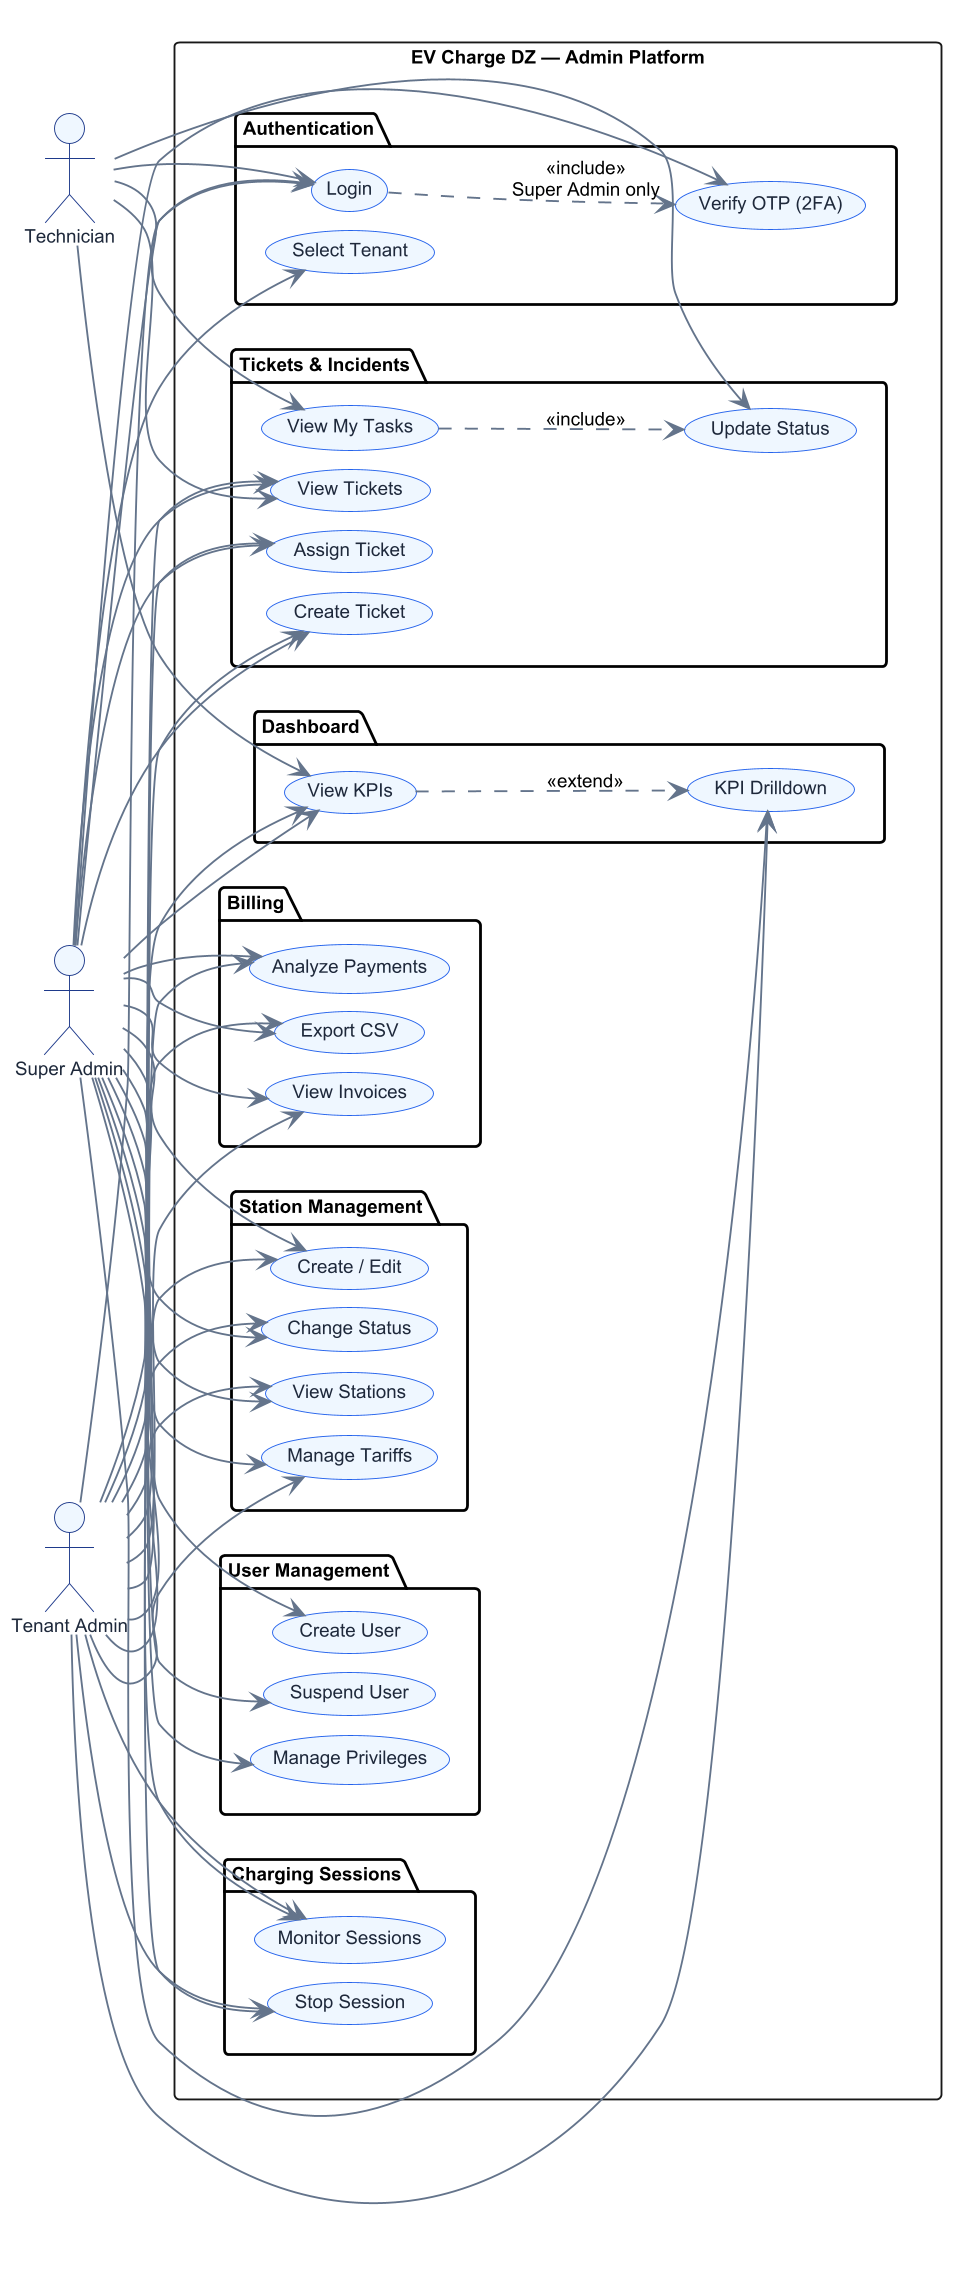
\includegraphics[width=0.72\textwidth, height=0.92\textheight, keepaspectratio]{../diagramme/UseCaseDiag.png}
  \caption{Use Case Diagram --- EV Charge DZ Admin Platform}
  \label{fig:usecase-diagram}
\end{figure}

% ──────────────────────────────────────────────────────────────────────────────
\section{Technical Constraints}

\subsection{Protocol Constraint --- OCPP~1.6}

The platform must implement OCPP~1.6 for station communication~\autocite{ocpp16_ed2}. As
established in Chapter~2, OCPP~2.0.1 was evaluated but excluded due to limited hardware
availability and network infrastructure maturity in Algeria.

\subsection{Regulatory and Market Constraints}

All billing must be expressed in Algerian Dinars~(DZD). Payment integration must support the
CIB interbank card network and local e-payment services, reflecting the payment landscape
available to Algerian EV operators and end users.

\subsection{Network Infrastructure Constraints}

Given variable connectivity conditions in certain Algerian deployment areas, the frontend must
retain functionality in partial offline scenarios. Operators must not lose access to operational
data during temporary backend outages.

% ──────────────────────────────────────────────────────────────────────────────
\section{Conclusion}

This chapter has established the complete requirements baseline for the EV Charge Manager
platform. Ten functional requirements and six non-functional requirements, combined with three
categories of technical and regulatory constraints, define the scope and boundaries of the
system. These requirements directly inform the architectural choices presented in Chapter~4 and
are validated by the implementation demonstrated in Chapter~5.

%%%=============================================================================
%%  CHAPTER 4 — CONCEPTION
%%%=============================================================================

\chapter{EV Charge Manager --- Architecture and Design}

This chapter presents the architectural and design decisions for EV Charge Manager, translating
the requirements established in Chapter~3 into a concrete technical blueprint. We describe the
general three-tier architecture, the multi-tenant isolation model, the data model, the user
access control structure, the authentication flow, and the technology stack selected for the
implementation.

% ──────────────────────────────────────────────────────────────────────────────
\section{General Architecture}

The platform follows a standard three-tier architecture:

\begin{itemize}
  \item \textbf{Presentation Tier}: A single-page application (SPA) built with React~18 and
        TypeScript~\autocite{react_docs, typescript_docs}, bundled with Vite~\autocite{vite_docs}. It
        runs entirely in the browser and communicates with the backend over HTTP/JSON.

  \item \textbf{Logic Tier}: A Node.js REST API built with Express.js~\autocite{nodejs_express},
        responsible for authentication, data validation, and business logic.

  \item \textbf{Data Tier}: A MySQL~8 relational database~\autocite{mysql_docs} storing all
        operational data (stations, sessions, tickets, billing records, users).
\end{itemize}

The frontend communicates with the backend via a centralized API client module. All requests are
authenticated using JSON Web Tokens (JWT)~\autocite{rfc7519}. The application is designed to
degrade gracefully: when the backend is unreachable, it falls back to locally persisted data
(browser \texttt{localStorage}) and notifies the operator with a visible offline-mode banner.

% ──────────────────────────────────────────────────────────────────────────────
\section{Technology Stack}

\begin{table}[h!]
  \centering
  \caption{EV Charge Manager --- Technology Stack}
  \label{tab:tech-stack}
  \renewcommand{\arraystretch}{1.3}
  \begin{tabular}{>{\bfseries}p{3.8cm} p{4cm} p{5.5cm}}
    \toprule
    Layer              & Technology            & Role \\
    \midrule
    Language           & TypeScript~5          & Type-safe JavaScript~\autocite{typescript_docs} \\
    UI Framework       & React~18              & Component-based SPA~\autocite{react_docs} \\
    Build Tool         & Vite~5                & Fast dev server and bundler~\autocite{vite_docs} \\
    UI Components      & shadcn/ui + Radix~UI  & Accessible component primitives \\
    Styling            & Tailwind CSS          & Utility-first CSS~\autocite{tailwindcss_docs} \\
    Charts             & Recharts              & SVG-based data visualisation~\autocite{recharts_docs} \\
    Routing            & React Router~v6       & Client-side navigation~\autocite{reactrouter_docs} \\
    Map                & Leaflet / OpenStreetMap & Interactive station map \\
    Backend            & Node.js + Express.js  & REST API server~\autocite{nodejs_express} \\
    Database           & MySQL~8               & Relational data storage~\autocite{mysql_docs} \\
    Authentication     & JWT + OTP (2FA)       & Stateless token auth~\autocite{rfc7519} \\
    Charging Protocol  & OCPP~1.6              & Station communication~\autocite{ocpp16_ed2} \\
    \bottomrule
  \end{tabular}
\end{table}

% ──────────────────────────────────────────────────────────────────────────────
\section{Multi-Tenant Architecture}

The platform supports multiple independent operators---referred to as \textit{tenants}---each
with complete data isolation. Two tenants are currently configured:

\begin{itemize}
  \item \textbf{Sonelgaz}: Algeria's national electricity company and primary EV infrastructure
        operator.
  \item \textbf{SAEIG}: A private EV charging network operator.
\end{itemize}

Tenant isolation is enforced at the database level through a \texttt{tenant\_id} foreign key on
all operational entities (stations, sessions, tickets, billing records, and users). At the
application level, a \textit{TenantContext} React context propagates the active tenant across
all components, which filter their data accordingly. Each tenant may also define custom branding
(accent color, logo), providing a white-label experience while sharing common platform
infrastructure.

% ──────────────────────────────────────────────────────────────────────────────
\section{Data Model}

The class diagram in Figure~\ref{fig:class-diagram} presents the database-oriented data model
of EV Charge Manager. The central entities are \texttt{Station}, \texttt{Session},
\texttt{Ticket}, \texttt{Invoice}, and \texttt{User}, each carrying a \texttt{tenant\_id}
foreign key that enforces the multi-tenant isolation described in the previous section.
Stations are linked to Sessions (one-to-many), and Sessions aggregate into Invoice records. The
\texttt{Ticket} entity references both a \texttt{Station} and an assigned \texttt{User}
(technician), and carries a full activity log for audit purposes.

\begin{landscape}
\begin{figure}[p]
  \centering
  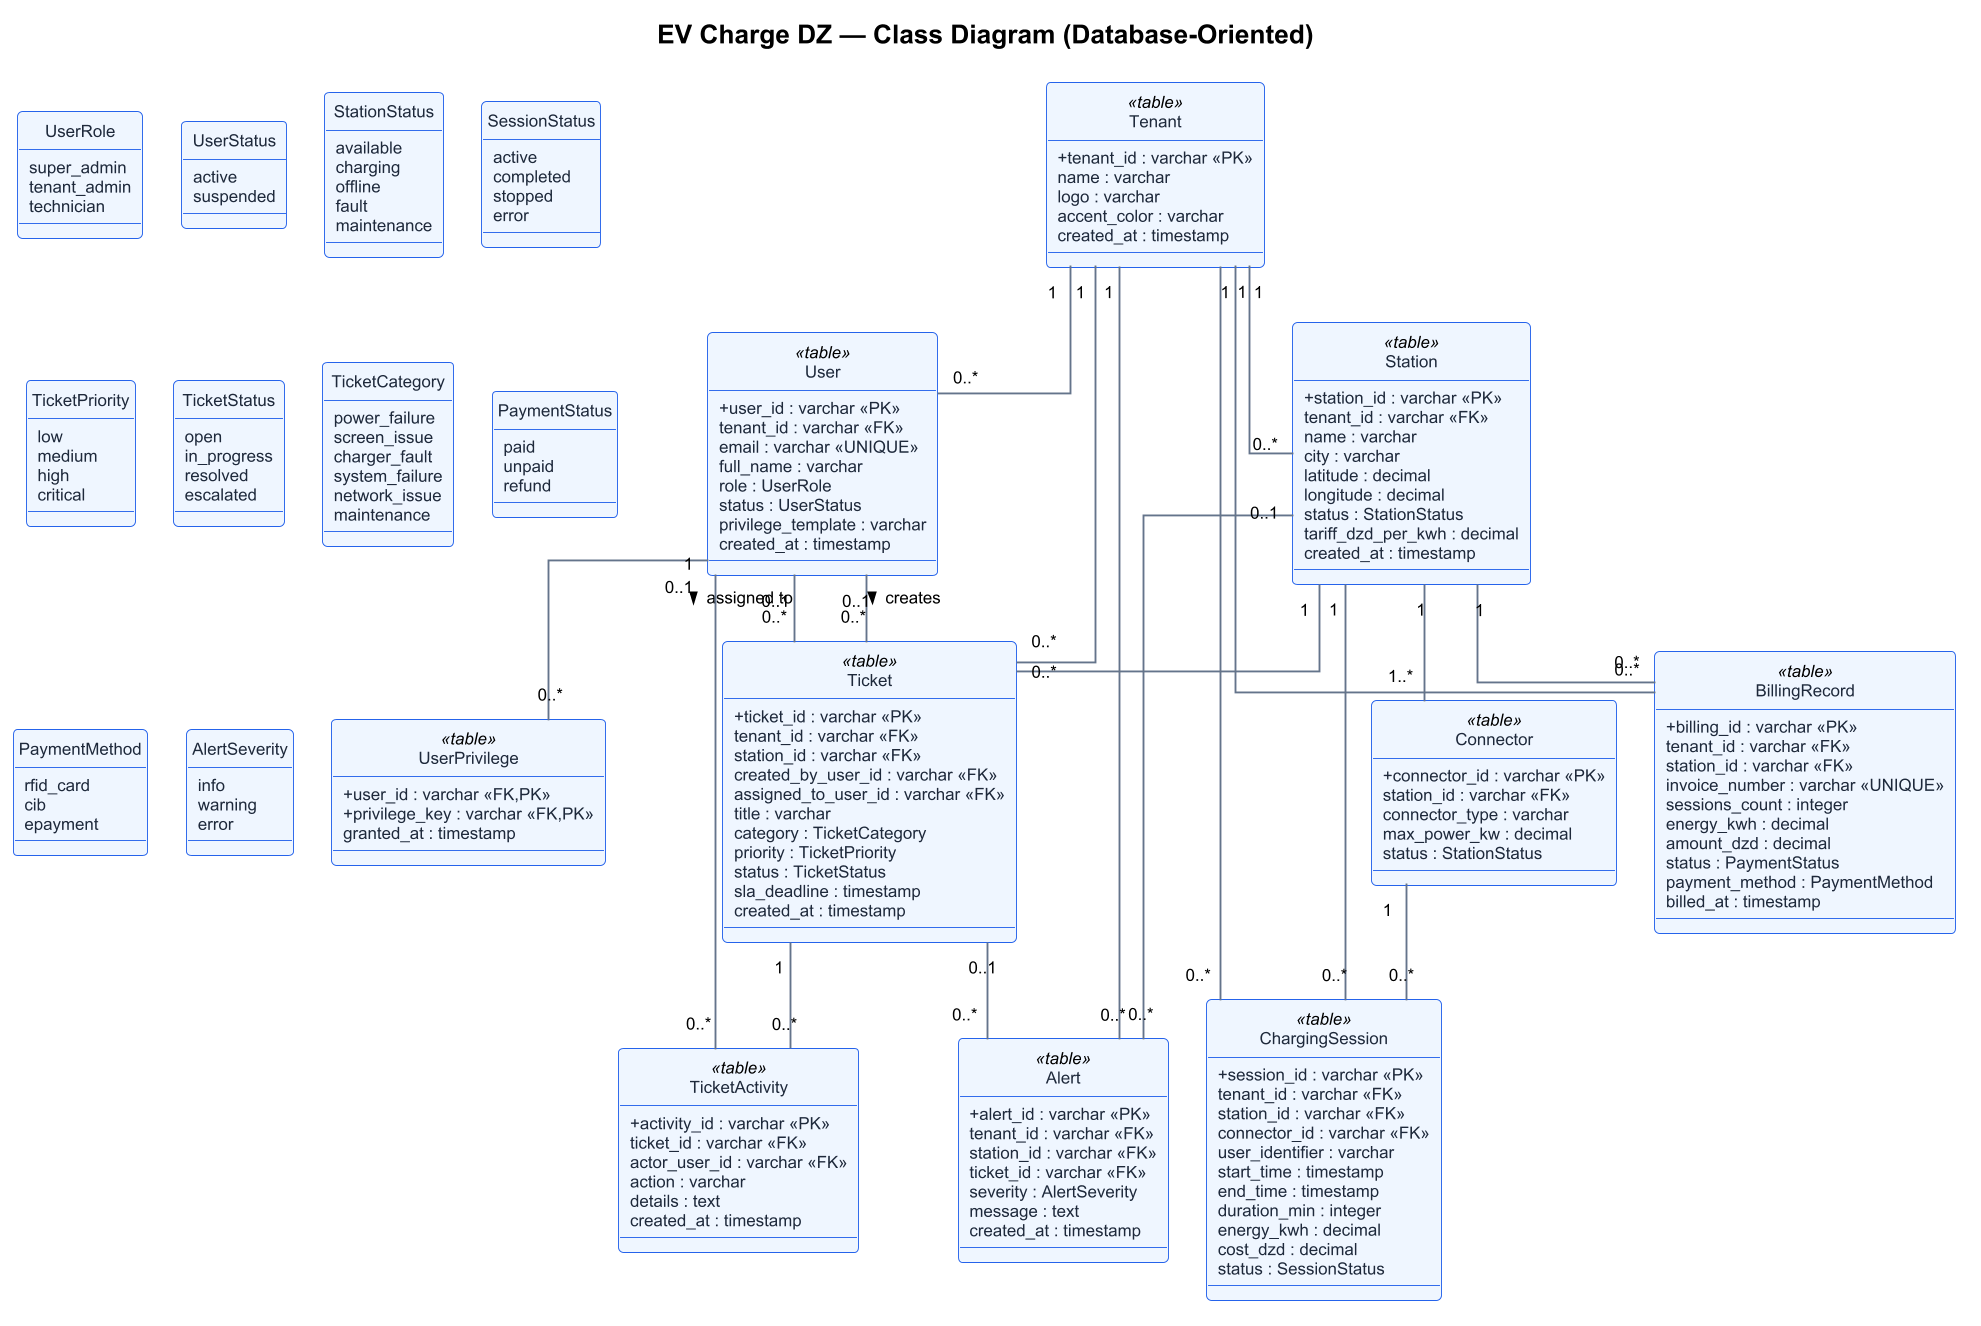
\includegraphics[width=\linewidth, height=0.88\textheight, keepaspectratio]{../diagramme/ClassDiag.png}
  \caption{Class Diagram --- EV Charge DZ (Database-Oriented)}
  \label{fig:class-diagram}
\end{figure}
\end{landscape}

% ──────────────────────────────────────────────────────────────────────────────
\section{User Roles and Access Control}

The platform implements Role-Based Access Control (RBAC) with three distinct user roles:

\begin{table}[h!]
  \centering
  \caption{User Roles and Module Access}
  \label{tab:user-roles}
  \renewcommand{\arraystretch}{1.3}
  \begin{tabular}{>{\bfseries}p{3.2cm} p{3cm} p{7cm}}
    \toprule
    Role           & Scope           & Accessible Modules \\
    \midrule
    super\_admin   & All tenants     & Dashboard, Stations, Sessions, Billing, Tickets,
                                       Users, Archives \\
    tenant\_admin  & Own tenant only & Dashboard, Stations, Sessions, Billing, Tickets \\
    technician     & Own tasks only  & My Tasks (assigned maintenance tickets) \\
    \bottomrule
  \end{tabular}
\end{table}

Beyond role assignment, the platform supports thirteen fine-grained privilege types
(e.g., \texttt{stations\_manage}, \texttt{billing\_view}, \texttt{reports\_export}), organized
into five templates for rapid onboarding: \textit{standard\_admin}, \textit{operations\_admin},
\textit{finance\_admin}, \textit{technician\_default}, and \textit{custom}. Routes in the
frontend are guarded by a \texttt{RequireAuth} component that verifies both authentication and
role before rendering any protected page.

% ──────────────────────────────────────────────────────────────────────────────
\section{Authentication Design}

User authentication follows a two-factor flow:

\begin{enumerate}
  \item The user submits their email, password, and tenant identifier on the login screen.
  \item The backend validates the credentials and generates a One-Time Password~(OTP) sent to
        the registered email address.
  \item The user enters the OTP on a dedicated verification screen. On successful validation,
        the backend issues a signed JWT~\autocite{rfc7519}.
  \item All subsequent API requests include the JWT as a \texttt{Bearer} token in the HTTP
        \texttt{Authorization} header. The backend validates the token signature and tenant
        claims on every protected endpoint.
\end{enumerate}

The JWT is stored in the browser's \texttt{localStorage} and is cleared on logout. The
\texttt{RequireAuth} component performs a client-side token presence check and role verification
before rendering any dashboard route. The sequence diagram in Figure~\ref{fig:seq-auth}
illustrates the complete authentication and OTP verification flow for a super administrator.

\begin{figure}[p]
  \centering
  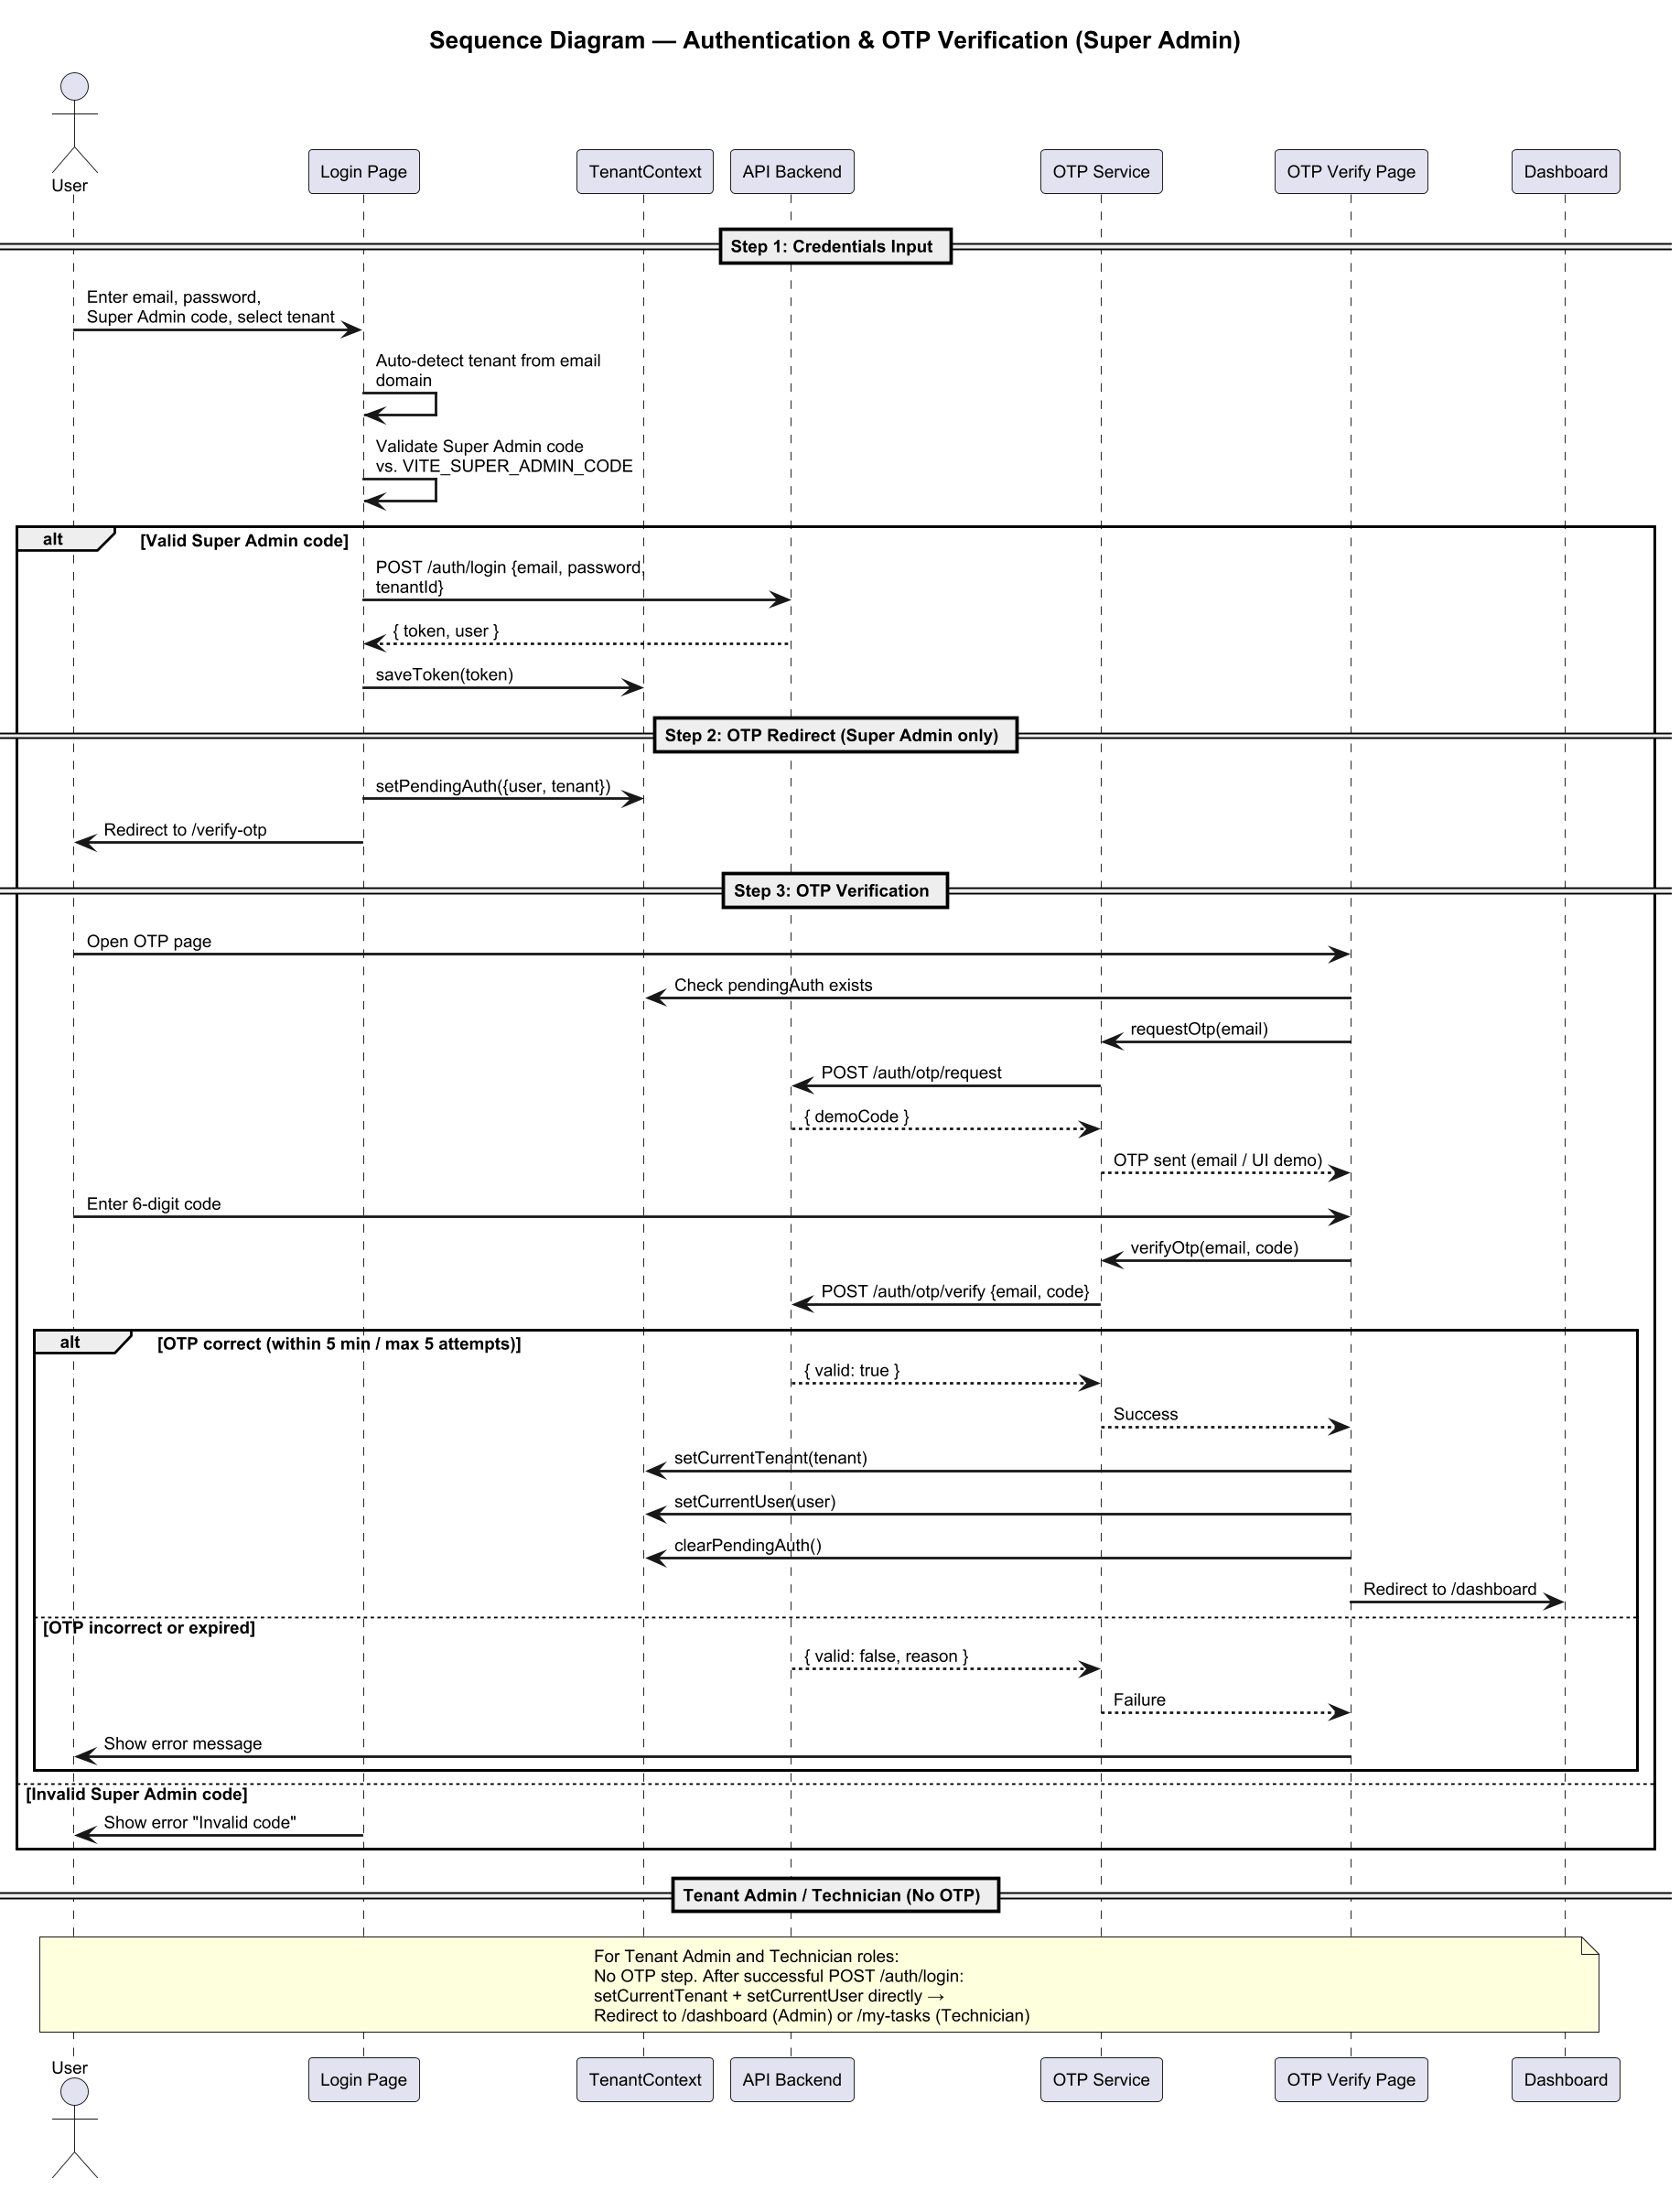
\includegraphics[width=\textwidth, height=0.92\textheight, keepaspectratio]{../diagramme/SeqAuth.png}
  \caption{Sequence Diagram --- Authentication and OTP Verification Flow (Super Admin)}
  \label{fig:seq-auth}
\end{figure}

% ──────────────────────────────────────────────────────────────────────────────
\section{Conclusion}

The architectural choices presented in this chapter --- three-tier separation, tenant-scoped
database isolation, RBAC with thirteen fine-grained privileges, and two-factor JWT
authentication --- directly address the functional and non-functional requirements identified in
Chapter~3. Together they constitute the technical blueprint for the platform implementation
detailed in Chapter~5.

%%%=============================================================================
%%  CHAPTER 5 — RÉALISATION ET TESTS
%%%=============================================================================

\chapter{EV Charge Manager --- Réalisation et Tests}

This chapter presents the concrete implementation of EV Charge Manager, module by module. Each
section describes the operational interface and behaviour of a functional component, demonstrating
how the design decisions of Chapter~4 translate into a working charging management platform. We
also describe the development environment and conclude with a comprehensive platform summary.

% ──────────────────────────────────────────────────────────────────────────────
\section{Development Environment}

The platform was developed on Windows~11 using Node.js~18~LTS for the backend runtime,
MySQL~8 Community Edition as the database server, and the Vite development server for the
React frontend. Visual Studio Code was used as the primary integrated development environment,
with ESLint and Prettier extensions enforcing code style consistency across the codebase. Git
was used for version control, with the project repository hosted on GitHub.

% ──────────────────────────────────────────────────────────────────────────────
\section{Dashboard Module}

The dashboard provides a real-time overview of the entire charging network through seven Key
Performance Indicators (KPIs), displayed as interactive cards:

\begin{itemize}
  \item \textbf{Active Stations}: Stations in \textit{available} or \textit{charging} status.
  \item \textbf{Offline Stations}: Stations in \textit{fault} or \textit{offline} status.
  \item \textbf{Under Maintenance}: Stations in \textit{maintenance} mode.
  \item \textbf{Active Sessions}: Currently ongoing charging sessions.
  \item \textbf{Energy Delivered}: Total energy dispatched (kWh) over the selected period.
  \item \textbf{Revenue}: Cumulative billing amount (DZD) over the selected period.
  \item \textbf{Network Uptime}: Weighted average station availability rate (\%).
\end{itemize}

Each KPI card displays a trend indicator comparing the current period to the previous one, and
supports a clickable drilldown that opens a contextual side panel. The dashboard also includes:

\begin{itemize}
  \item A 30-day revenue and energy trend chart (multi-line chart built with
        Recharts~\autocite{recharts_docs}).
  \item A connector-type distribution chart (donut chart showing CCS2\,/\,CHAdeMO\,/\,Type~2
        share).
  \item A 24-hour energy consumption curve (hourly resolution).
  \item A real-time alerts feed categorized by severity (info, warning, error).
\end{itemize}

A date filter (Today\,/\,7~Days\,/\,30~Days) is persisted in \texttt{localStorage} to maintain
operator preferences across sessions.

% ──────────────────────────────────────────────────────────────────────────────
\section{Station Management Module}

The Stations module provides complete lifecycle management for charging infrastructure. It offers
two complementary views:

\begin{itemize}
  \item \textbf{Table View}: A searchable, filterable table with filters for status and city.
  \item \textbf{Map View}: An interactive Leaflet/OpenStreetMap map showing each station as a
        color-coded marker (by operational status). Clicking a marker reveals station details.
\end{itemize}

\subsection{Connector Standards}

Each station may host multiple connector types simultaneously. The platform supports the three
main standards deployed in Algeria and internationally:

\begin{table}[h!]
  \centering
  \caption{Supported EV Connector Standards}
  \label{tab:connectors}
  \renewcommand{\arraystretch}{1.3}
  \begin{tabular}{>{\bfseries}p{2.5cm} p{2cm} p{3cm} p{5cm}}
    \toprule
    Type      & Current & Typical Power  & Use Case \\
    \midrule
    CCS2      & DC      & Up to 350\,kW  & Fast and ultra-fast DC charging \\
    CHAdeMO   & DC      & Up to 400\,kW  & Japanese DC standard \\
    Type~2    & AC      & 3.7--22\,kW    & AC home and public slow charging \\
    \bottomrule
  \end{tabular}
\end{table}

\subsection{Station Status Values}

Stations cycle through five operational states: \textit{available} (idle, ready),
\textit{charging} (session active), \textit{offline} (network lost), \textit{fault} (hardware
or software fault detected via OCPP~\autocite{ocpp16_ed2}), and \textit{maintenance} (under
scheduled service).

\subsection{Station Actions}

Operators can: enable a station, disable it, toggle maintenance mode, update the tariff
(DZD/kWh), and create a new station with GPS coordinates selected via an embedded location
picker map. All status-changing actions require confirmation through a modal dialog and are
logged in the system audit trail. A CSV export function allows operators to download the
current filtered station list for external reporting.

% ──────────────────────────────────────────────────────────────────────────────
\section{Session Monitoring Module}

The Sessions module provides a chronological log of all charging sessions associated with the
active tenant. Each session record contains: a unique session identifier, the source station
name, the connector used, the user's identifier (RFID tag or account ID), session start time,
duration (minutes), energy delivered (kWh), billing amount (DZD), and final status.

Session status values are: \textit{active} (ongoing), \textit{completed} (ended normally),
\textit{stopped} (manually interrupted by user or operator), or \textit{error} (abnormal
termination). Operators can filter sessions by status and station, and export results to CSV.

% ──────────────────────────────────────────────────────────────────────────────
\section{Billing Module}

The Billing module tracks all financial transactions generated by charging sessions. It supports
three payment methods common in the Algerian market:

\begin{itemize}
  \item \textbf{RFID Card}: The most widely deployed method; the customer authenticates using
        an RFID tag registered to their account.
  \item \textbf{CIB (Carte Interbancaire)}: Electronic payment via the Algerian interbank bank
        card network.
  \item \textbf{E-Payment}: Mobile wallet or online payment gateway.
\end{itemize}

Each billing record includes an invoice number, associated station, number of sessions
aggregated, total energy consumed (kWh), total amount (DZD), payment status (paid, unpaid, or
refund), and the payment processing timestamp. The module provides per-method performance
statistics, including transaction count, success rate, failed transaction count, average
processing time (seconds), and revenue contribution percentage.

% ──────────────────────────────────────────────────────────────────────────────
\section{Maintenance Ticket System}

The Ticket module implements a structured fault-reporting and maintenance-scheduling workflow.
When a station issue is detected---automatically via the alert system or manually by an
operator---a ticket is created with the following attributes:

\begin{itemize}
  \item \textbf{Category}: One of six types---power failure, screen issue, charger fault,
        system failure, network issue, or scheduled maintenance.
  \item \textbf{Priority}: Low, medium, high, or critical.
  \item \textbf{SLA Deadline}: A contractual resolution deadline tracked and displayed as a
        countdown; breached deadlines trigger automatic escalation.
  \item \textbf{Assignment}: The ticket is assigned to a specific technician.
  \item \textbf{Activity Log}: Every status change, comment, and action is recorded with a
        timestamp and actor identity, providing a complete audit trail.
\end{itemize}

The ticket lifecycle follows four states, as illustrated in Figure~\ref{fig:activity-ticket}:
\textit{open} $\rightarrow$ \textit{in\_progress} $\rightarrow$ \textit{resolved}
(or \textit{escalated} if the SLA deadline is breached without resolution).

Technicians access their work queue through the dedicated \textit{My Tasks} page, which
displays only tickets assigned to the currently logged-in user, allowing them to focus
exclusively on their own workload without visibility into unrelated tickets.

\begin{figure}[p]
  \centering
  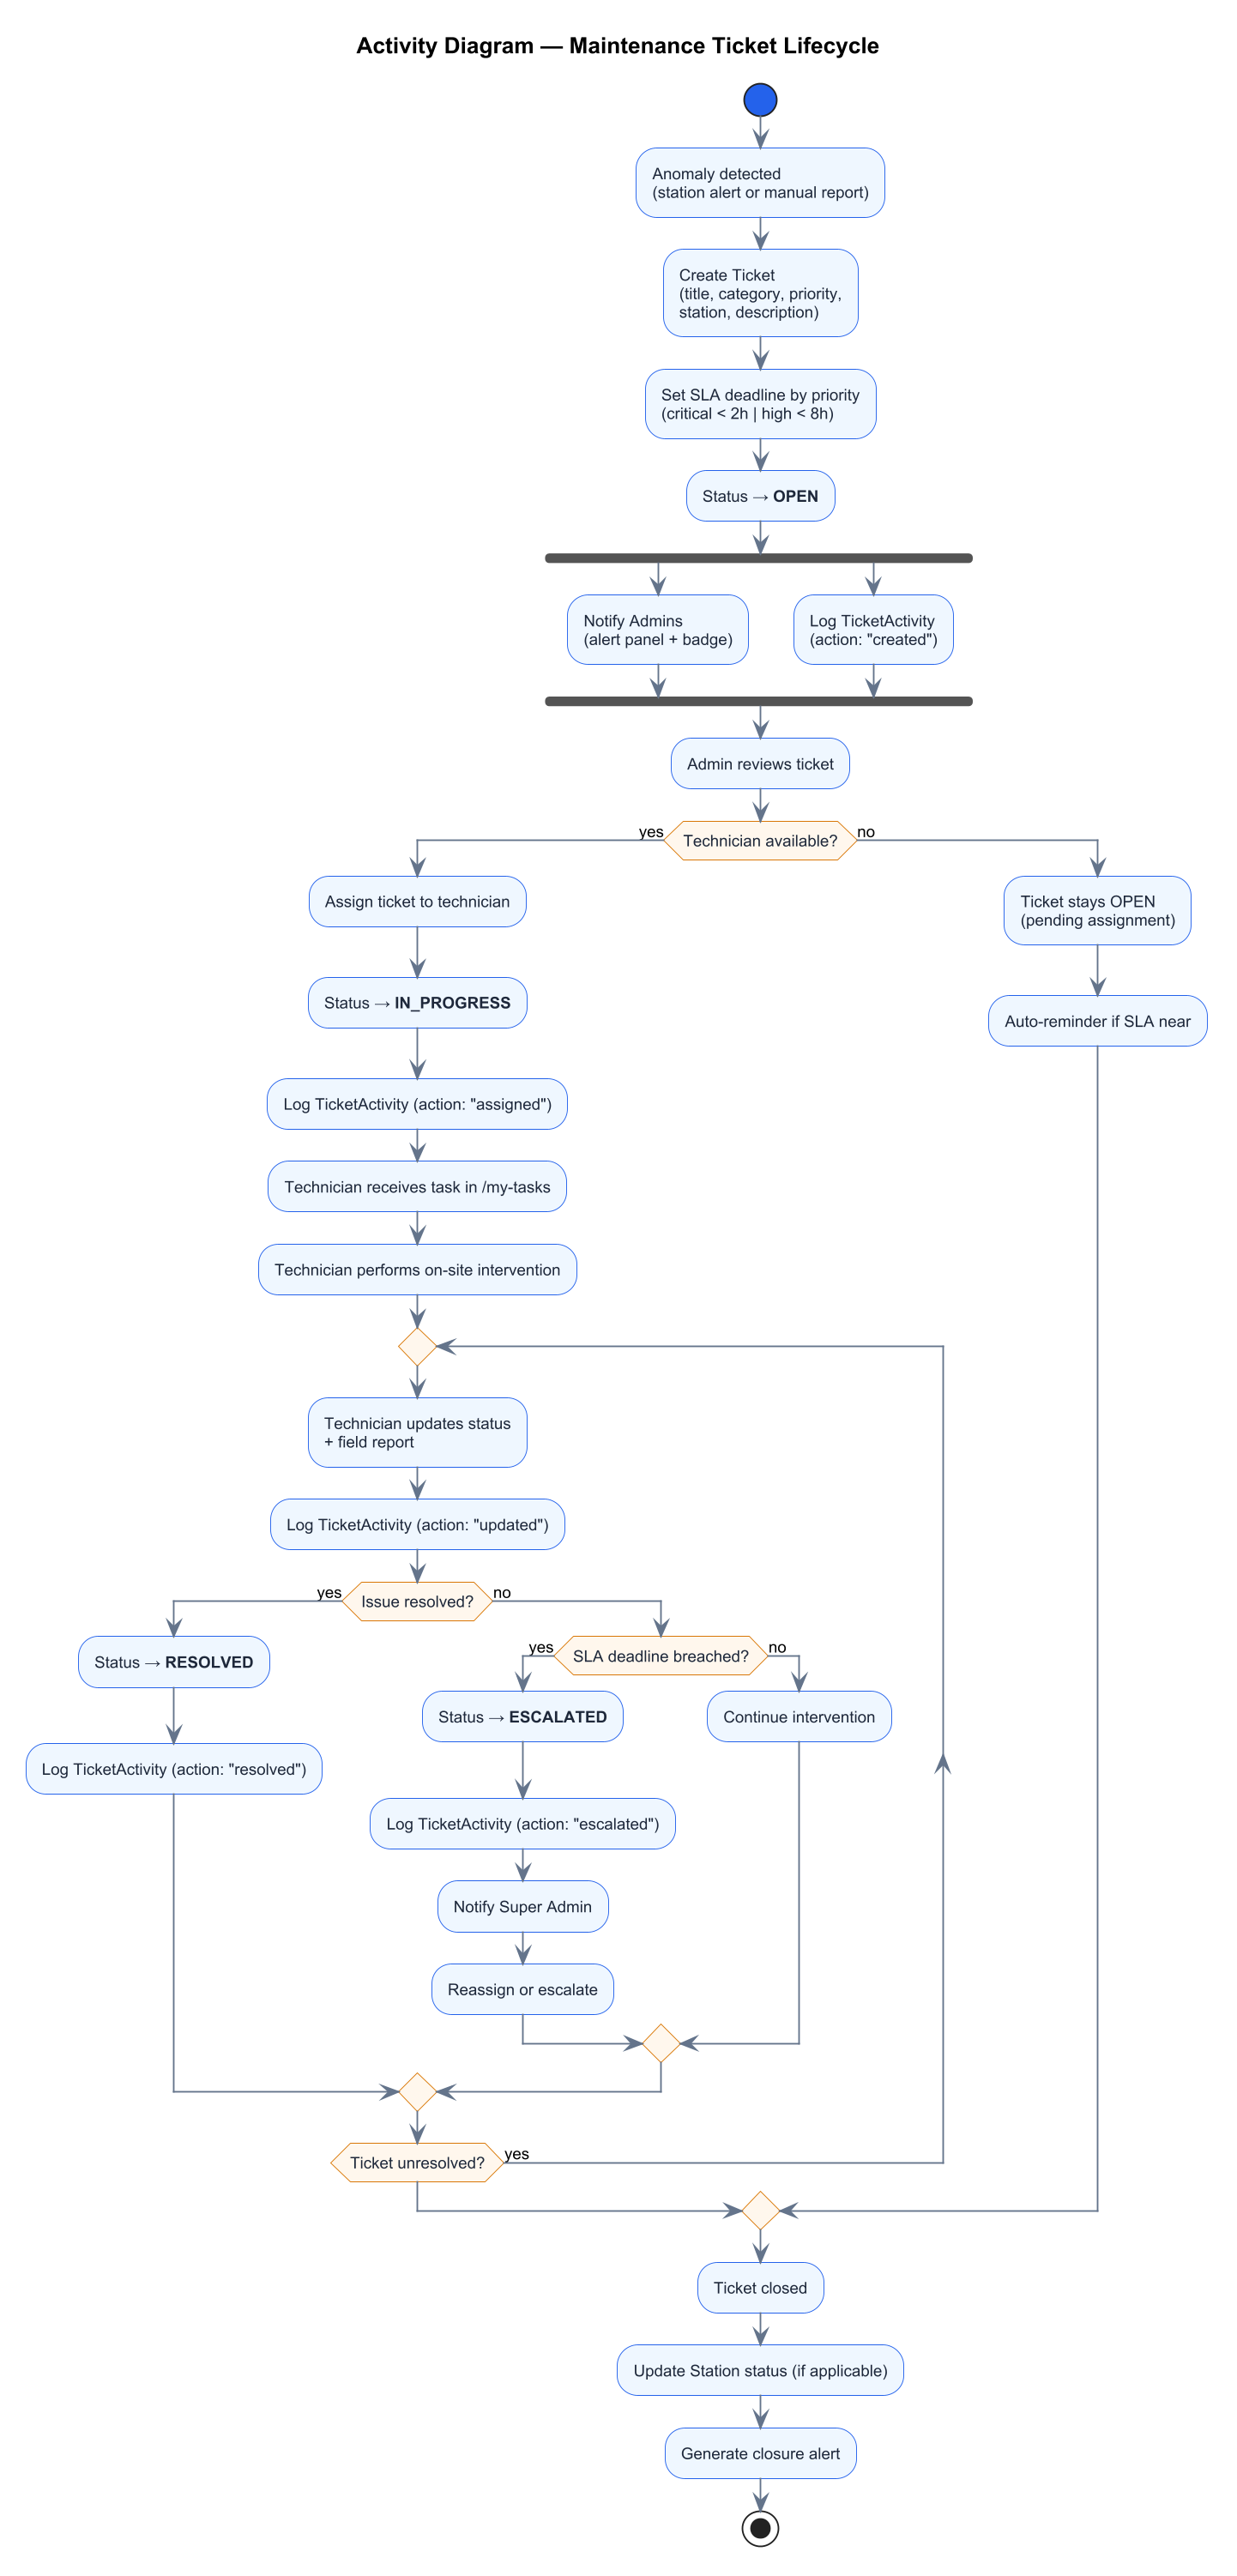
\includegraphics[width=0.62\textwidth, height=0.92\textheight, keepaspectratio]{../diagramme/ActivityTicket.png}
  \caption{Activity Diagram --- Maintenance Ticket Lifecycle}
  \label{fig:activity-ticket}
\end{figure}

% ──────────────────────────────────────────────────────────────────────────────
\section{User Management Module}

The User Management module, accessible to super\_admin accounts only, allows the creation,
modification, and suspension of platform users. When creating a user, the administrator assigns:
a role (super\_admin, tenant\_admin, or technician), a tenant affiliation, and a privilege
template. Templates automatically assign the thirteen available privilege flags appropriate for
the selected operational profile, while the \textit{custom} template allows manual selection of
individual privileges.

User accounts can be suspended (blocking login without deletion) and reactivated, providing
full lifecycle management of operator personnel.

% ──────────────────────────────────────────────────────────────────────────────
\section{Data Resilience and Offline Mode}

A key architectural decision is the platform's graceful degradation strategy. The frontend
checks for the presence of a backend API base URL at startup. When the backend is unreachable
(network failure or server downtime), the application falls back to data persisted in the
browser's \texttt{localStorage} and displays a prominent offline-mode notification banner.
This ensures operators retain read access to station lists, recent session records, and ticket
data even during connectivity interruptions.

% ──────────────────────────────────────────────────────────────────────────────
\section{Platform Summary}

\begin{table}[h!]
  \centering
  \caption{EV Charge Manager --- Platform Specification Summary}
  \label{tab:platform-summary}
  \renewcommand{\arraystretch}{1.3}
  \begin{tabular}{>{\bfseries}p{4.5cm} p{9cm}}
    \toprule
    Aspect                & Detail \\
    \midrule
    Platform Type         & Multi-tenant SaaS web application \\
    Target Market         & Algeria (Sonelgaz and SAEIG operators) \\
    Charging Protocol     & OCPP~1.6~\autocite{ocpp16_ed2} \\
    User Roles            & super\_admin, tenant\_admin, technician \\
    Granular Privileges   & 13 privilege types across 5 templates \\
    Authentication        & Email\,/\,password + OTP (2FA) + JWT~\autocite{rfc7519} \\
    Supported Connectors  & CCS2, CHAdeMO, Type~2 \\
    Payment Methods       & RFID card, CIB, e-payment \\
    Billing Currency      & Algerian Dinar (DZD) \\
    Frontend              & React~18 + TypeScript + Vite~\autocite{react_docs, vite_docs} \\
    Backend               & Node.js + Express.js~\autocite{nodejs_express} \\
    Database              & MySQL~8~\autocite{mysql_docs} \\
    Map                   & Leaflet / OpenStreetMap \\
    Offline Resilience    & localStorage fallback with graceful degradation \\
    \bottomrule
  \end{tabular}
\end{table}

% ──────────────────────────────────────────────────────────────────────────────
\section{Conclusion}

EV Charge Manager's implementation fulfils all ten functional requirements identified in
Chapter~3 and follows the architecture designed in Chapter~4. The seven operational
modules --- dashboard, station management, session monitoring, billing, maintenance tickets,
user management, and offline resilience --- collectively deliver a production-ready charging
management solution adapted to Algeria's EV infrastructure context. The platform provides a
complete, locally adapted response to the gap identified in the introduction, and establishes
a solid foundation for the future enhancements described in the general conclusion.

%%%=============================================================================
%%  GENERAL CONCLUSION
%%%=============================================================================

\chapter*{General Conclusion and Perspectives}
\addcontentsline{toc}{chapter}{General Conclusion and Perspectives}

This thesis has presented the design and implementation of EV Charge Manager, a multi-tenant
web platform for managing electric vehicle charging infrastructure in Algeria. The work
demonstrates that a robust, scalable charging management solution can be built using modern
open-source web technologies while remaining aligned with international charging standards.

The platform successfully delivers:

\begin{itemize}
  \item A multi-tenant architecture supporting independent operators with complete data isolation
        and custom branding.

  \item Role-based access control covering three distinct operational profiles: platform
        administrator, tenant administrator, and field technician, with thirteen fine-grained
        privilege flags.

  \item A real-time operational dashboard with seven KPIs, interactive charts, and drilldown
        panels for fleet-level insight.

  \item Complete station lifecycle management, including multi-connector configuration,
        geographic mapping via OpenStreetMap, and OCPP-aligned status tracking~\autocite{ocpp16_ed2}.

  \item A structured maintenance ticket system with SLA enforcement, priority levels, technician
        assignment, and complete audit trails.

  \item Multi-method billing support for RFID cards, CIB bank cards, and e-payment, with
        per-method performance analytics.

  \item A resilient frontend architecture that falls back to locally cached data when the backend
        is unreachable, ensuring operational continuity.
\end{itemize}

\textbf{Future Perspectives}

Several enhancements can extend the platform's capabilities in future iterations:

\begin{enumerate}
  \item \textbf{OCPP~2.0.1 Migration}: Upgrading to OCPP~2.0.1~\autocite{ocpp201} would enable
        native ISO~15118 Plug\,\&\,Charge integration, dynamic smart charging profiles, and
        bidirectional V2G energy flows.

  \item \textbf{AI-Powered Predictive Maintenance}: Integrating machine learning models for
        fault prediction based on historical ticket data and session anomalies would reduce mean
        time to repair (MTTR).

  \item \textbf{Mobile Companion Application}: A dedicated mobile app for EV drivers to locate
        stations, view real-time availability, book charging slots, and manage payments.

  \item \textbf{Smart Grid Integration}: Real-time communication with the national grid
        (Sonelgaz) to enable demand response, photovoltaic surplus absorption, and peak-load
        shaving aligned with the capabilities described in Chapter~1~\autocite{iso15118_2022}.

  \item \textbf{Algerian Payment Gateway Integration}: Direct connection to local payment
        processors (BaridiMob, CIB online) for automated invoice collection.
\end{enumerate}

EV Charge Manager represents a first concrete step towards a comprehensive, locally adapted EV
charging ecosystem for Algeria. Its technical foundation---built on open standards and modern
cloud-ready architecture---provides the flexibility to evolve alongside the country's growing
electric mobility infrastructure.

%%%=============================================================================
%%  BIBLIOGRAPHY
%%%=============================================================================

\clearpage
\printbibliography[
  heading = bibintoc,          % add "References" to the table of contents
  title   = {References},
]

\end{document}
